
\chapter{Pilot study}\label{chap:pilot_study}

Having defined our system, we carry out an initial study of the frictional properties. First, we evaluate the numerical results for a non-cut sheet in order to define suitable metrics for a numerical evaluation of friction and justify some of the default parameter choices. This provides a basis for the following study where we consider the Tetrahedron and Honeycomb Kirigami patterns as well. We conduct a more systematic investigation of the friction dependencies to temperature, sliding speed, spring constant and timestep. Finally, we consider the mean friction of all three configurations when stretched. This includes an analysis of the dependence to contact area and the friction-load curves. 


\section{Friction simulation parameters}
The \acrshort{MD} simulations we will carry out to measure friction are governed
by a small set of parameters. For the purpose of creating a machine learning we
need to standardize these parameters. This we keep most of them constant with
only a small subset of parameters being varied: sheet configuration, strain and
load. Instead of starting with the parameter selection process, we first state
the final choice in \cref{tab:final_param}. Due to the great number of
parameters, we do not make an exhaustive search of all parameters before
deciding on the final settings. Instead, we take a basis in parameters used in
similar friction simulations \cite{li_evolving_2016, Yoon2015MolecularDS,
liu_high-speed_2014, zhu_study_2018, ma12091425} and adjust accordingly to the
aim of getting stable measurements and reducing computation time where possible.
Parameters such as initial relaxation time, pauses and strain speed are chosen
mainly from the results of initial stability tests. The sheet and pull block
sizes are chosen with a consideration of the balance between Kirigami design
options and computational resources. The scan direction is chosen to be parallel
to the connection line between the pull blocks. This is mainly chosen in order
to avoid unessecary complexity in the motion since it can be hypethesized that the
center of the sheet can drag behind for other scan directions. The remaining
parameters: Temperature $T$, sliding speed $v_{\text{slide}}$, spring constant
$K$, normal load $F_N$, timestep $dt$ and sliding distance have been chosen
because the friction output remains relatively stable with moderate
perturbations around these default values. We will explain this in more detail
later in the chapter. Note that the default values in \cref{tab:final_param}
will be used when nothing else is stated explicitly.


\begin{table}[H]
  \begin{center}
  \caption{Parameters involved for the numerical \acrshort{MD} simulation for measuring friction. The default values correspond to the final choice used for the dataset. The shaded cells denote the parameters varied in the \acrshort{ML} dataset.}
  \label{tab:final_param}
  \begin{tabular}{ | C{4cm} | C{3.5cm} | X{6cm}|} \hline
    \textbf{Parameter} & \textbf{Default value} &  \textbf{Description} \\ \hline
    $T$ & \SI{300}{K} &  Temperature of the system. \\ \hline
    $v_{\text{slide}}$ &\SI{20}{m/s} & Sliding speed for the sheet translation. \\ \hline
    $K$ & $\infty$ & Spring constant for the coupling between the virtuel atom and the sheet pull blocks. \\ \hline
    Scan direction & $(x,y) = (0,1)$ \mbox{(zigzag direction)}  & The direction for which we translate the sheet. \\ \hline   
    \cellcolor{black!7} Sheet configuration & \cellcolor{black!7} Contiguous & \cellcolor{black!7} Binary mapping describing which atoms are removed (0) and which is still present (1) in the graphene sheet.  \\ \hline
    \cellcolor{black!7} Strain amount & \cellcolor{black!7} [0, rupture] & \cellcolor{black!7} The ratio of change in length to the original length. \\ \hline
    \cellcolor{black!7} $F_N$ & \cellcolor{black!7} [0.1, 10] nN & \cellcolor{black!7} Applied normal force to the pull blocks. \\ \hline
    $dt$ & \SI{1}{fs} &  \acrshort{MD} integration timestep. \\ \hline
    Initial relaxation time &  \SI{15}{ps} & Initial relaxation time before straining. \\ \hline
    Pauses & \SI{5}{ps} & Relaxation pauses after strain, and during the normal load phase (before translating the sheet). \\ \hline
    Strain Speed & \SI{0.01}{ps^{-1}} & The rate of straining for the sheet. \\ \hline
    Slide distance & \SI{400}{Å} & How far the sheet is translated. \\ \hline
    Sheet size & $130.029 \times \SI{163.219}{\text{Å}}$ & Spatial 2D size of the sheet.  \\ \hline
    Pull block size & $2 \times 130.029 \times \SI{15.183}{\text{Å}}$ & Spatial 2D size of the pull blocks. \\ \hline
  \end{tabular}
  \end{center}
\end{table}

%

% We aim to chose the parameters in order to accomodate a balance between generlizable and stable result which is simmutaneously a suting candidate as a proof of concept for the control of friction properties using kirigami inspired cuts. 



% Due to the great number of parameters, and corresponding range of reasonable numerical values they can take, it is ... to parameter search including all of these. Thus, we will to a great extent rely on a reverse engineering in order to establish a set of parameters for the \textit{physical} and \textit{measurement} categories along with numerical ranges for the $\textit{ML input}$ category which gives stable and promising results. By doing so we effectively narrow down the parameter regime for which the investigated frictional properties belong. We aim to chose the parameters in order to accomodate a balance between generlizable and stable result which is simmutaneously a suting candidate as a proof of concept for the control of friction properties using kirigami inspired cuts. 

% In the following we present the results of the friction simulations in parallel to the procedure of investigating the choice of different parameters. 

% In the following subsections (X to Y) we are going to present the friction simulation results in parallel to the presentation of the reasoning behind the parameter choices. For this we will refer to the default parameter choice showcased in \cref{tab:final_param} which is representative of the final parameter choices. 




% The sliding velocity is 20 m/s, which is comparable to the operating conditions in micromechanical systems (MEMS), but which is much larger than the typical velocity in scanning force microscopy (SFM) experiments. \cite{mo_friction_2009} Supplementary materials.


% We should try to set the physcis and measurement parameters in such a way that we reduce computation speed where it is doesn't infer with the frictional properties study.



% Parameters expected to have a physical effect on the friction properties, which is kept fixed and thus not included in the machine learning input set. 

% Paramters influecing the simulation kinetics and being representative of the experimental procedure that we are mimicking. These parameters is chosen with the aim of getting stable parameters under small perturbations of the given parameter. 

% The remaining paramters serves as input variables for optimization process and is thus given as input variables for the machine learning (ML).




% Say someting about how these parameters is chosen. Reference to articles for which these was mirrored from. 





% We need to define some ranges for the ML input paramters. $F_N$, stretch ranges where it is not prone to ruptures. The configuration it self does not have clear rules but is also being regulated by the no rupture requirement. 

% Retardation effects due to the finiteness of the speed of sound are usually irrelevant in slow-speed experiments (v < 1 mm/s) \cite{Manini_2016}

% In macroscopic tribology experiments, sliding speeds often range in the 0.1 − 10 m/s region \cite{Manini_2016}

% By contrast, in nanoscale AFM experiments the tip usually advances at much lower speeds $\sim$ 1 $\mu$m/s: over a typical run it is possible to simulate a tiny ∼ 1 pm displacement, far too small to explore even a single atomic-scale event, let alone averaging over a steady state.\cite{Manini_2016}


% However, MD simulations can provide so much physical insight that they make sense even if carried out at much higher speeds than in real-life AFM or surface force apparatus (SFA) experiments: in practice, currently the sliding speeds of most atomistic tribology simulations are in the $\sim$ 1 m/s region.\cite{Manini_2016}


% Besides the limitations of system size and simulation times that are obvious and will be discussed later, there is another limitation concerning temperature, that is rarely mentioned. All classical frictional simulations, atomistic or otherwise, are only valid at sufficiently high temperature. They become in principle invalid at low temperatures where the mechanical degrees of freedom of solids progressively undergo ”quantum freezing”, and both mechanics and thermokinetics deviate from classical. \cite{Manini_2016}.




% \newpage
% Single friction simulation analysis
\section{Force traces}\label{sec:single_analysis}
We begin by assessing the friction force traces, i.e.\ force vs.\ time curves, for a single friction simulation using the default parameters shown in \cref{tab:final_param} for a non-cut sheet with
no stretch applied and a normal load of $\SI{1}{nN}$. 


\subsection{Force oscillations}\label{sec:force_oscillations}
We evaluate the friction force as the force acting on the sheet from the
substrate. We consider initially the force component $F_{\parallel}$ parallel
to the drag direction as plotted in \cref{fig:drag_Ff}. We use a sample rate of
10 ps$^{-1}$ = 100 timesteps$^{-1}$ for which each sample is the mean value of
the preceding 100 timesteps. We observe immediately that the data carries oscillations on different time scales which match our general expectations for
sliding involving periodic surfaces. By applying a Savgol filter to the data
with a polynomial order of 5 and a window length of 150 timesteps (corresponding to a
sliding distance of 3 Å or a time window of 15 ps) we can qualitatively point
out at least two different frequencies of oscillation. During the first 10 Å of
sliding, seen in \cref{fig:drag_Ff_10}, we see roughly three waves on the Savgol
filter corresponding to a relatively high frequency, while for the duration of
100 Å of sliding, seen in \cref{fig:drag_Ff_100}, the same Savgol filter reveals
a lower frequency on top, creating the visual pattern of a wavepacket. The data
does not indicate clear signs of stick-slip behavior as otherwise found in
other studies, e.g.\ by Zhu and Li \cite{zhu_study_2018} for graphene on gold,
who saw a more typical saw tooth shape in the force trace. Besides the difference
in the substrate material, using gold instead of silicon, they used a lower sliding
speed of \SI{10}{m/s} and a soft spring of $K = \SI{10}{N/m}$. By adopting these
parameters we get a slightly different force trace behavior as shown in
\cref{fig:drag_Ff_10_K10_v10} and \cref{fig:drag_Ff_100_K10_v10}. This change
breaks the symmetry in the force oscillations but still does not produce any
significant discontinuities in the trace. By keeping the spring constant $K =
\SI{10}{N/m}$ and lowering the sliding speed further down to \SI{1}{m/s} we are
able to demonstrate a proper stick-slip behavior as shown in
\cref{fig:drag_Ff_10_K10_v1} and \cref{fig:drag_Ff_100_K10_v1}. Considering all
three simulations we might classify the results from the default settings, $K =
\inf, v = \SI{20}{m/s}$, as smooth sliding,  $K = \SI{10}{N/m}, v =
\SI{10}{m/s}$, as a transition phase with possible occasional slipping, and $K
= \SI{10}{N/m}, v = \SI{1}{m/s}$ as certain stick-slip behaviour. This confirms the qualitative observation the stick-slip behavior is suppressed with stiff springs~\cite{bonelli_atomistic_2009} springs and high sliding velocity~\cite{liu_high-speed_2014}. Having a low sliding speed comes with a high computational cost which is the reason that we choose a relatively high sliding speed of \SI{20}{m/s}. The choice of an infinite spring constant is related to the stability of the measurements and is discussed later in this chapter \hl{make sure it is, maybe make a reference}.


%
%
% Working here
%
%

\begin{figure}[H]
  \centering
  \begin{subfigure}[t]{0.49\textwidth}
      \centering
      \includegraphics[width=\textwidth]{figures/baseline/drag_Ff_10Å.pdf}
      \caption{$K = \inf$, $v = \SI{20}{\frac{m}{s}}$ (10 Å sliding).}
      \label{fig:drag_Ff_10}
  \end{subfigure}
  \hfill
  \begin{subfigure}[t]{0.49\textwidth}
      \centering
      \includegraphics[width=\textwidth]{figures/baseline/drag_Ff_100Å.pdf}
      \caption{$K = \inf$, $v = \SI{20}{\frac{m}{s}}$ (100 Å sliding).}
      \label{fig:drag_Ff_100}
    \end{subfigure}
    \hfill
    \begin{subfigure}[t]{0.49\textwidth}
      \centering
      \includegraphics[width=\textwidth]{figures/baseline/drag_Ff_10Å_K10_v10.pdf}
      \caption{$K = \SI{10}{\frac{N}{m}}$, $v = \SI{10}{\frac{m}{s}}$ (10 Å sliding).}
      \label{fig:drag_Ff_10_K10_v10}
    \end{subfigure}
    \hfill
    \begin{subfigure}[t]{0.49\textwidth}
      \centering
      \includegraphics[width=\textwidth]{figures/baseline/drag_Ff_100Å_K10_v10.pdf}
      \caption{$K = \SI{10}{\frac{N}{m}}$, $v = \SI{10}{\frac{m}{s}}$ (100 Å sliding).}
      \label{fig:drag_Ff_100_K10_v10}
  \end{subfigure}
  \hfill
    \begin{subfigure}[t]{0.49\textwidth}
      \centering
      \includegraphics[width=\textwidth]{figures/baseline/drag_Ff_10Å_K10_v1.pdf}
      \caption{$K = \SI{10}{\frac{N}{m}}$, $v = \SI{1}{\frac{m}{s}}$ (10 Å sliding).}
      \label{fig:drag_Ff_10_K10_v1}
    \end{subfigure}
    \hfill
    \begin{subfigure}[t]{0.49\textwidth}
      \centering
      \includegraphics[width=\textwidth]{figures/baseline/drag_Ff_100Å_K10_v1.pdf}
      \caption{$K = \SI{10}{\frac{N}{m}}$, $v = \SI{1}{\frac{m}{s}}$ (100 Å sliding).}
      \label{fig:drag_Ff_100_K10_v1}
  \end{subfigure}
  \hfill
     \caption{Force traces of the friction force $F_\parallel$ with respect to the drag direction between acting from the substrate on the full sheet and substrate. The force traces is plotted against the sliding distance (lower x-axis) and thr corresponding sliding time (upper x-axis). The sliding distance is measured by displacement of the virtual atom tethering the sheet. The red line represents a Savgol filter with window polynomial order 5 and window length of 150 timesteps (corresponding to a sliding distance of 3 Å or a time window of 15 ps). Each row, (a,b), (c,d), (e,f), represents a different choice of the spring constant $K$ and sliding speed $v$, while the columns show the same result for two different time scales. The default settings are represented in figure (a) and (b).}
     \label{fig:drag_Ff}
\end{figure}

By performing a Fourier Transform on the data, using the default parameters, we can quantify the leading frequencies observed in figure \cref{fig:drag_Ff_10} and \cref{fig:drag_Ff_100}. The Fourier transform is shown in \cref{fig:ft_a}, and by plotting the two most dominant frequencies $f_1 = 0.0074$ ps$^{-1}$ and $f_2 = 0.0079$ ps$^{-1}$ as a sine sum, $\sin{(2\pi f_1)} + \sin{(2\pi f_2)}$, we find a qualitatively convincing fit to the observed wavepacket shape as seen in \cref{fig:ft_b}. We can convert the frequencies according to that of a wavepacket. By using the trigonometric identity
\begin{align*}
\sin (a+b) &= \sin (a) \cos (b) + \cos (a) \sin (b), \\
\sin (a-b) &= \sin (a) \cos (b) - \cos (a) \sin (b),
\end{align*}
and decomposing the frequencies as $f_1 = a - b$, $f_2 = a + b$, we can rewrite the sine sum as the sinusoidal product
\begin{align*}
  \sin(2\pi f_1) + \sin(2\pi f_2) &= \sin\big(2\pi (a - b)\big) + \sin\big(2\pi (a + b)\big) \\
  &= \sin(2\pi a)\cos(2\pi b) + \cancel{\cos(2\pi a)\sin(2\pi b)} + \sin(2\pi a)\cos(2\pi b) - \cancel{\cos(2\pi a)\sin(2\pi b)} \\
  &= 2 \sin(2\pi a) \cos(2\pi b),
\end{align*} 
with 
\begin{align*}
  a = \frac{f_1 + f_2}{2} &= 0.0763 \pm \SI{0.0005}{ps^{-1}},& 
  b = \frac{f_2 - f_1}{2} &= 0.0028 \pm \SI{0.0005}{ps^{-1}},& \\
  &= 0.381 \pm \SI{0.003}{{\text{Å}}^{-1}},& 
  &= 0.014 \pm \SI{0.003}{{\text{Å}}^{-1}}.& 
\end{align*}
In the latter transition we have denoted the frequency with respect to the sliding distance by considering the default sliding speed of $\SI{20}{m/s} = \SI{0.2}{\text{Å}/ps}$. This
makes us recognize the high osccilation frequency as $a$ and the low frequency
as $b$. The faster one has a period of $T_a = 2.62 \pm \SI{0.02}{\text{Å}}$ \footnote{The
uncertainty $\Delta y$ is calculated as $\Delta y = \left|\frac{\partial
y}{\partial x} \Delta x \right|$ for uncertainty $\Delta x$ and $y(x)$} which
corresponds well with the magnitude of the lattice spacing and especialy that of
graphene at 2.46 Å as expected theoretically. The longer period $T_b = 71 \pm
\SI{15}{\text{Å}}$ is not obviously explained. We noticed a similar long period osciallation for all three cases, \cref{fig:drag_Ff_100}, \cref{fig:drag_Ff_100_K10_v10} and \cref{fig:drag_Ff_100_K10_v1}, regarding stick-slip behaviour, and thus we not believe that this is directly related. The initial build up in friction force is reminiscent of a friction strengthening, which is often reported \hl{SOURCE}, but the periodicity goes against this idea. Instead, we might attribute it to some kind of phonon
resosnance which could be a physical phenonama or simply a feature of our
\acrshort{MD} modelling. 

\begin{figure}[H]
  \centering
  \begin{subfigure}[t]{0.49\textwidth}
    \centering
    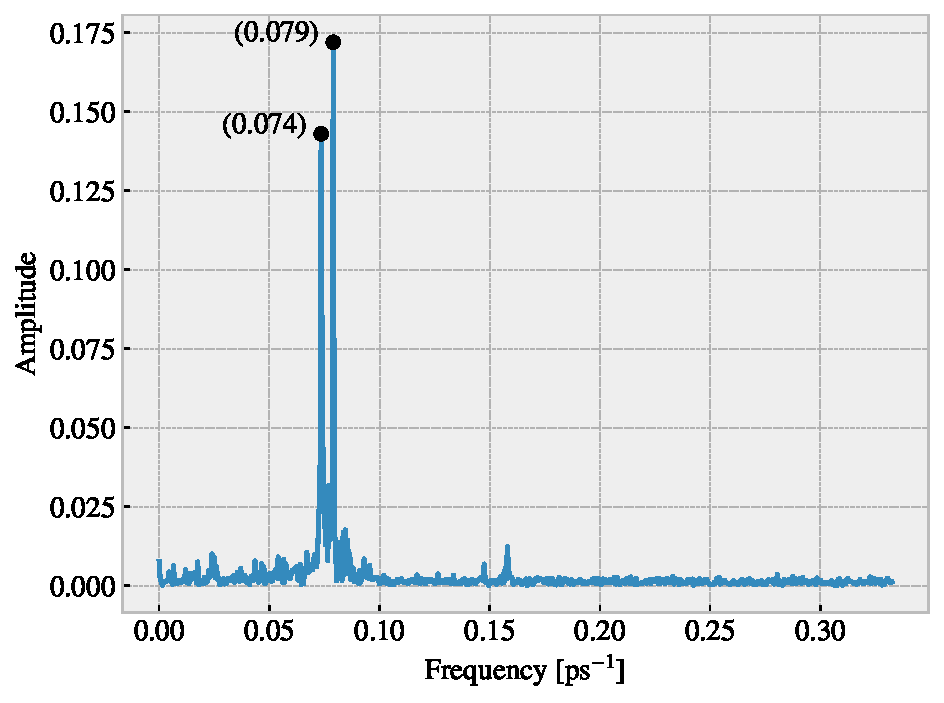
\includegraphics[width=\textwidth]{figures/baseline/ft_zoom.pdf}
    \caption{FT result shown for a reduced frequency range.}
    \label{fig:ft_a}
  \end{subfigure}
  \hfill
  \begin{subfigure}[t]{0.49\textwidth}
      \centering
      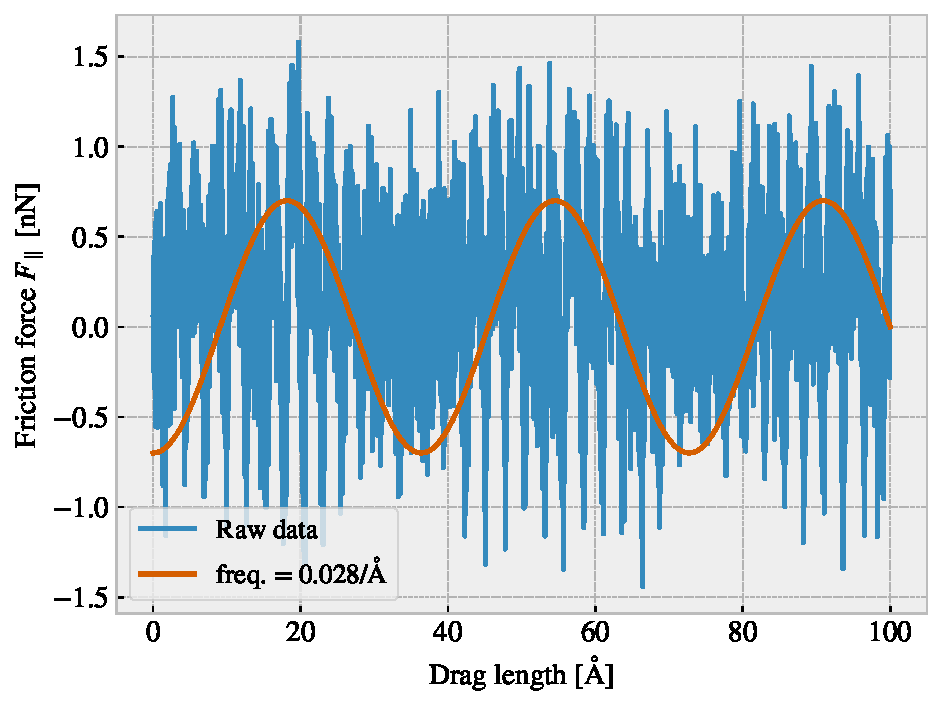
\includegraphics[width=\textwidth]{figures/baseline/ft_sine.pdf}
      \caption{Two most dominant frequencies applied to the data from \cref{fig:drag_Ff_100}}
      \label{fig:ft_b}
  \end{subfigure}
  \caption{Fourier transform analysis of the full friction force data (all 400 Å sliding distance) shown in \cref{fig:drag_Ff}. (a) shows the two most dominant frequency peaks. Note that no significant peaks was found in a higher frequency than included here. (b) shows a comparison between the raw data and the wavefunction corresponding to the two peaks in figure (a).}
  \label{fig:ft}
\end{figure}


\subsection{Decompositions}
In the previous analysis we have looked only at the friction force for the full
sheet, including the rigid pull blocks, and with
respect to the drag direction. We found this way of measuring the friction force to be the most intuitive and reliable, but we will present the underlying arguments for this choice in the following.

Due to the fact that we are only applying cuts to the inner sheet, and not the
pull blocks, it might seem more natural to only consider the friction on that
part. If the desired frictional properties can be achieved by altering the inner
sheet one can argue that any opposing effects from the pull blocks can be
mitigated by simply scaling the relative size between the inner sheet and the pull
blocks. However, when looking at the force traces decomposed with respect to the
inner sheet and pull block regions respectivly, see \cref{fig:decomp_group}, we
observe that the friction force arrising from those parts are seemingly
antisymmetric. That is, the distribution of the fricitonal pull from the
substrate on the sheet is oscillating between the inner sheet and the pull
block. Keeping in mind that normal force is only applied to the pull blocks we
might take this as an intrinsic feature of the system which does not nessecary dissapear by scaling of the spatial ratio between the inner sheet and pull block. Any interesting friciton properties might depend on this internal distribution of forces. Hence, we hedge our bets and use the full sheet friction force as a hollistic approach to avoid excluding relevant information in the measurement data.

Similar we might question the decision of
only considering the frictional force projected onto the sliding direction as
we are then neglecting the ``side shift'' induced during sliding. In \cref{fig:decomp_direc} we show the decomposition in terms of force components parallel $F_{\parallel}$ and perpendicular $F_{\perp}$ to the sliding direction respectively. We notice that the most dominant trend appears for the parallel component. If we want to include the perpendicular component as well we would have to evaluate friction as the length of the force vector instead, but this would remove the sign of the force direction and shift the mean friction force up as we clearly see both negative and positive contributions in the parallel force trace. One option to accommodate this issue is by using the vector length for the magnitude but keeping the sign from the parallel component. However, we omit such compromises as this might make the measurement interpretation unessercary complex, and we use only the parallel component going forward. 

\begin{figure}[H]
  \centering
  \begin{subfigure}[t]{0.49\textwidth}
    \centering
    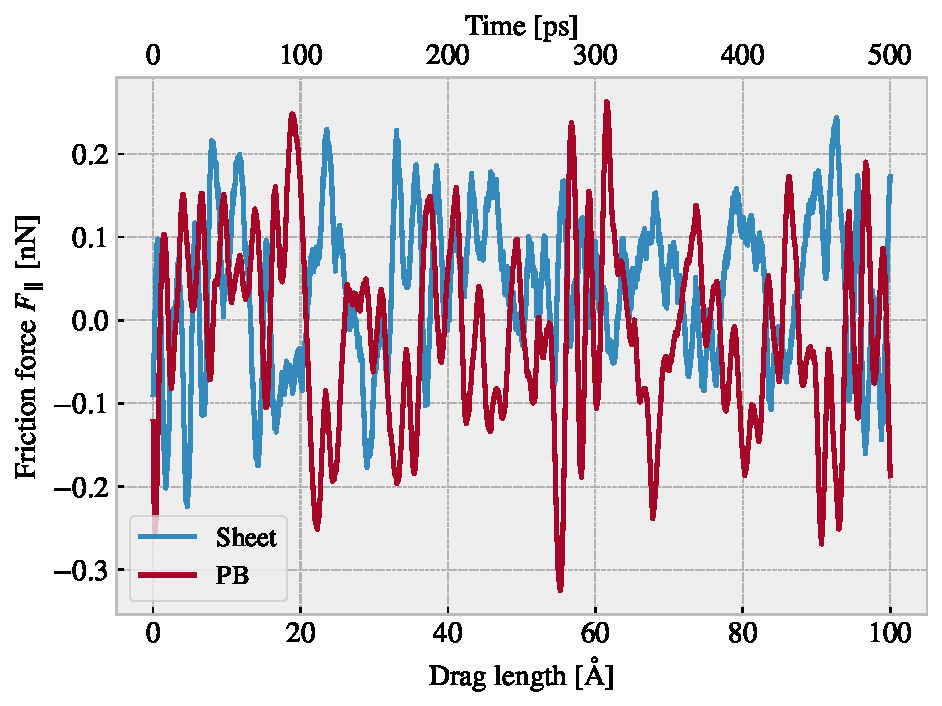
\includegraphics[width=\textwidth]{figures/baseline/decomp_group.pdf}
    \caption{}
    \label{fig:decomp_group}
  \end{subfigure}
  \hfill
  \begin{subfigure}[t]{0.49\textwidth}
      \centering
      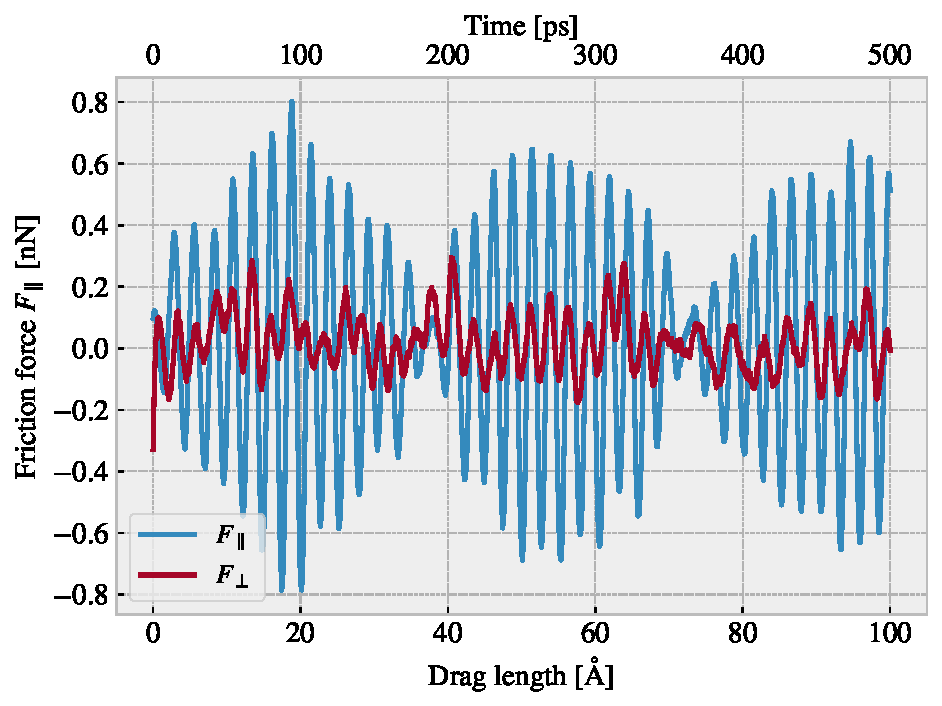
\includegraphics[width=\textwidth]{figures/baseline/decomp_direc.pdf}
      \caption{}
      \label{fig:decomp_direc}
  \end{subfigure}
  \caption{Friction force decomposition on the default parameter force trace shown in \cref{fig:drag_Ff} showing only the applied Savgol filters. (a) Decomposition into group inner sheet (sheet) and pull blocks (PB). (b) Decomposition into parallel ($F_{\parallel}$) and perpendicular ($F_{\perp})$ to drag sliding direction.}
  \label{fig:decomp}
\end{figure}


\subsection{Center of mass path}
From the previous observations of the force traces \cref{fig:drag_Ff} we
demonstarted both smooth sliding and stick-slip behaviour. Considering the force
decomposition in \cref{fig:decomp_direc} we know that the frictional forces in
the perpendicular direction to sliding is also present. By looking at the
$x,y$-position for the sheet Center of Mass (\acrshort{CM}) we see a qualitative
different behaviour when reconsidering the spring constant and sliding speed
investigated in \cref{fig:drag_Ff} which is shown in \cref{fig:CM_path}. The
default case in \cref{fig:CM_path_def} shows a rather straight path forward with
only a small side motion in comparison to the cases in
\cref{fig:CM_path_K10_v10} and \cref{fig:CM_path_K10_v1}. However, the
\acrshort{CM} accelerates and deaccelerates with a high frequency, much to high
to be associated with the lattice spaing on the order of 2.46 Å (interatomic
distance of 1.42 Å). One possible explanation is that the sheet and substrate
constitues an incommensurable contact for which travelling kink excitations make
the atoms move in such a way that the sheet \acrshort{CM} is incremented in
small ``burst''. When looking at the $K = \SI{10}{\frac{N}{m}}$, $v =
\SI{10}{\frac{m}{s}}$ case in \cref{fig:CM_path_K10_v10} we see a completely
different \acrshort{CM} path where the rapid parts alligns visually better with
the force oscialltiosn shown earlier in \cref{fig:drag_Ff_100_K10_v10}. The
\acrshort{CM} accelerates forward and the deaccelerates in combination with a
side motion that lead to the \acrshort{CM} path making a loop as it slows down.
Finally we have the $K = \SI{10}{\frac{N}{m}}$, $v = \SI{10}{\frac{m}{s}}$ in
\cref{fig:CM_path_K10_v10} which is confirmed to have stick-slip behaviour in
\cref{fig:drag_Ff_100_K10_v1}. Here the \acrshort{CM} path shows a more chaotic
movement between acceleration which also alligns visually well with the timing
of the slips seen in \cref{fig:drag_Ff_100_K10_v1}. The chaotic motion is not
obviously connected to the stick-slip motion, but we ommit a further
investigation as this is not corresponding to the parameters that we will be
using. 


\begin{figure}[H]
  \centering
  \begin{subfigure}[t]{0.85\textwidth}
    \centering
    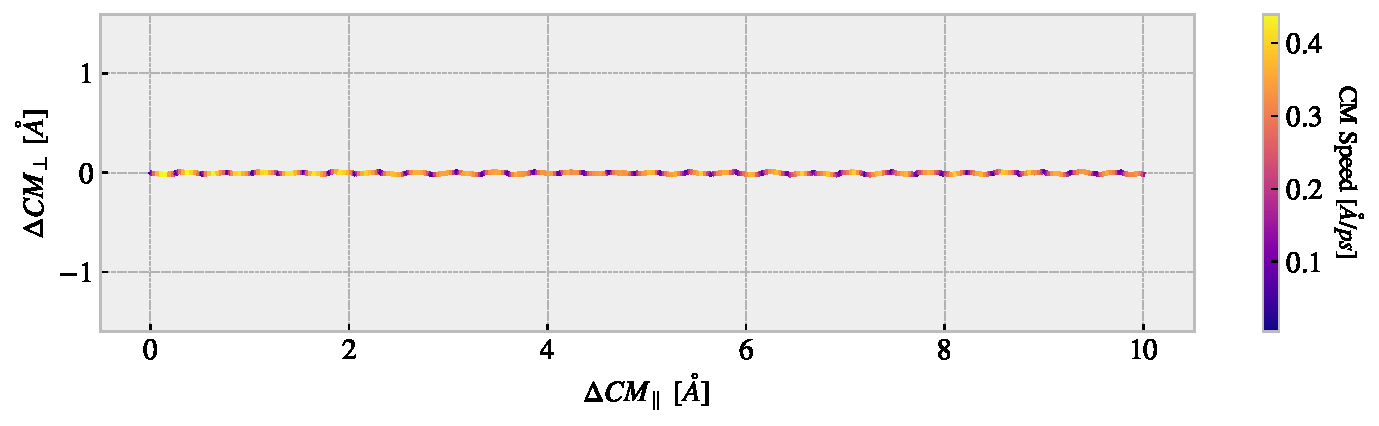
\includegraphics[width=\textwidth]{figures/baseline/COM_path_K0.pdf}
    \caption{$K = \inf$, $v = \SI{20}{\frac{m}{s}}$.}
    \label{fig:CM_path_def}
  \end{subfigure}
  \hfill
  \begin{subfigure}[t]{0.85\textwidth}
    \centering
    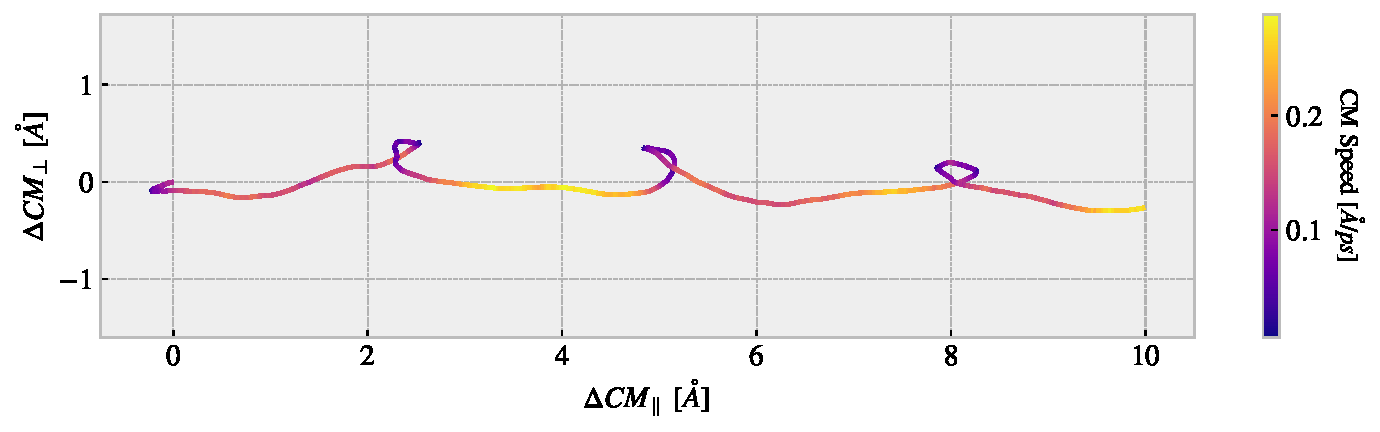
\includegraphics[width=\textwidth]{figures/baseline/COM_path_K10_v10.pdf}
    \caption{$K = \SI{10}{\frac{N}{m}}$, $v = \SI{10}{\frac{m}{s}}$.}
    \label{fig:CM_path_K10_v10}
  \end{subfigure}
  \begin{subfigure}[t]{0.85\textwidth}
    \centering
    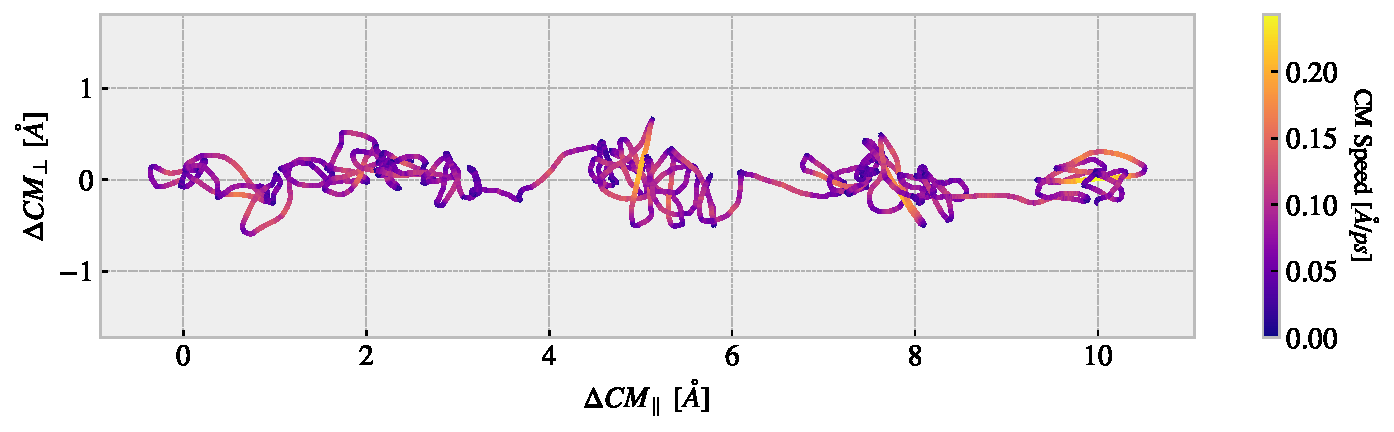
\includegraphics[width=\textwidth]{figures/baseline/COM_path_K10_v1.pdf}
    \caption{$K = \SI{10}{\frac{N}{m}}$, $v = \SI{1}{\frac{m}{s}}$.}
    \label{fig:CM_path_K10_v1}
  \end{subfigure}
  \caption{Center of Mass (\acrshort{CM}) position relative to the start of the sliding phase in terms of the direction parallel to the sliding direction $\Delta COM_{\parallel}$ and the axis perpendicular to the sliding direction $\Delta COM_{\perp}$. The colorbar denotes the absolute speed of the \acrshort{CM} motion. Figure a-c shows different parameters used for the spring constant $K$ and sliding speed $v$ similar to that used in \cref{fig:drag_Ff}. (a) Default: $K = \inf$, $v = \SI{20}{\frac{m}{s}}$. (b) $K = \SI{10}{\frac{N}{m}}$, $v = \SI{10}{\frac{m}{s}}$. (c) $K = \SI{10}{\frac{N}{m}}$, $v = \SI{1}{\frac{m}{s}}$ }
  \label{fig:CM_path}
\end{figure}


\section{Defining metrics for friction}\label{sec:fric_metrics}

In order to evaluate the frictional properties of the sheet we aim to reduce the force trace results, adressed in section \cref{sec:single_analysis}, into single metrics describing the kinetic and static friciton resepctively. 

\subsection{Kinetic friction}
We measure kinetic friction as the mean of the friction force trace. More
precisly, we take the mean value of the last half of the dataset in order to
ensure that we are sampling from a stable system. For a full sliding simulation
of 400 Å we thus base our mean value on the last 200 Å (1000 ps) of sliding.
In \cref{fig:runmean} we have shown the force trace for the first 10 Å of
sliding together with a 50\% running mean window. The choice of such a short sliding distance is merely to illustrate the samplig procedure,
and we see that the final mean estimate (marked
with a dot) takes a negative value due to the specific cut-off of the few
oscialltion captured here. Nonetheless, one approach to quanity the uncertainy
of the final mean estimate is to consider the variation of the running mean
preceeding the final mean value. The more the running mean fluctuates the more
uncertainty associated with the final estimate. Only the running mean
``close'' to the ending should be considered, since the first part will rely on
data from the beginning of the simulation. From the Fourier analyse in section \cref{sec:force_oscillations} we found the longest significant oscillation period to be $\sim \SI{71}{\text{Å}}$. Hence, we find it reasonable to use the standard deviation (\acrshort{std}) for the last $\sim \SI{71}{\text{Å}}$ of the running mean window to evaluate the fluctuations. When including the full sliding length this corresponds to the last $\sim 35 \%$ of the running mean window. We consider the \acrshort{std} as an estimate of the absolute error and calculate the relative error by a division of the final mean value. In \cref{fig:runstd} we showcase a
running relative error based on the \acrshort{std}, with a window of length
$35 \%$ the mean window, in a continuation of the illustrative case of a 10 Å
sliding from \cref{fig:runmean}. In this case we get an extremely high relative error of $\sim 257\%$, but this is desirable since the sampling period leads to an unphysical negative value which should be associated with a high uncertainty. 

\begin{figure}[H]
  \centering
  \begin{subfigure}[t]{0.49\textwidth}
    \centering
    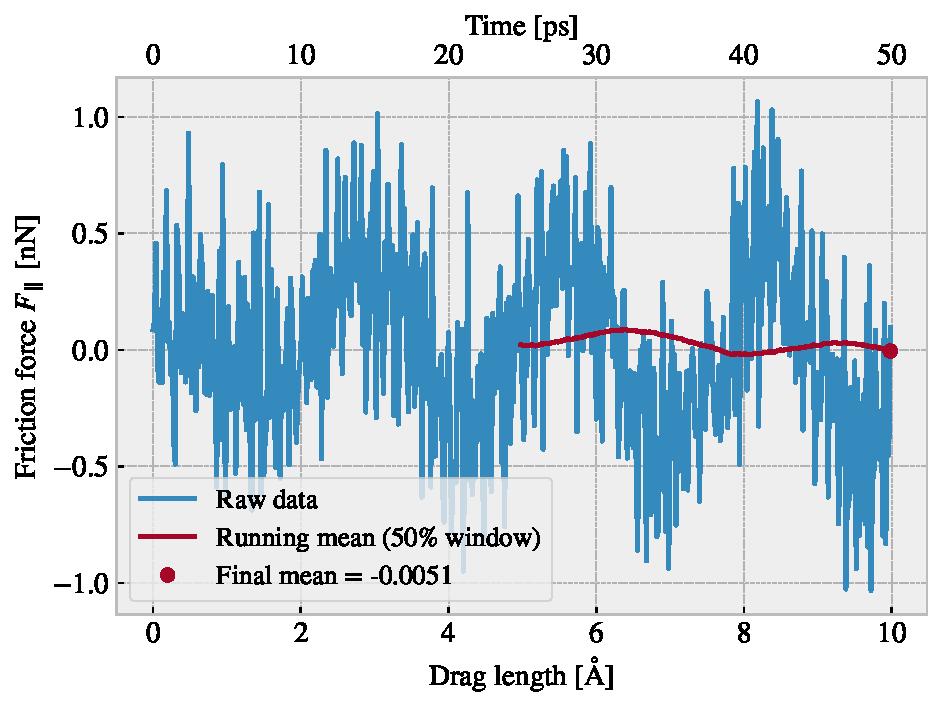
\includegraphics[width=\textwidth]{figures/baseline/Ff_runmean.pdf}
    \caption{Running mean with window length $\SI{5}{\text{Å}}$ (50\% the data length).}
    \label{fig:runmean}
  \end{subfigure}
  \hfill
  \begin{subfigure}[t]{0.49\textwidth}
      \centering
      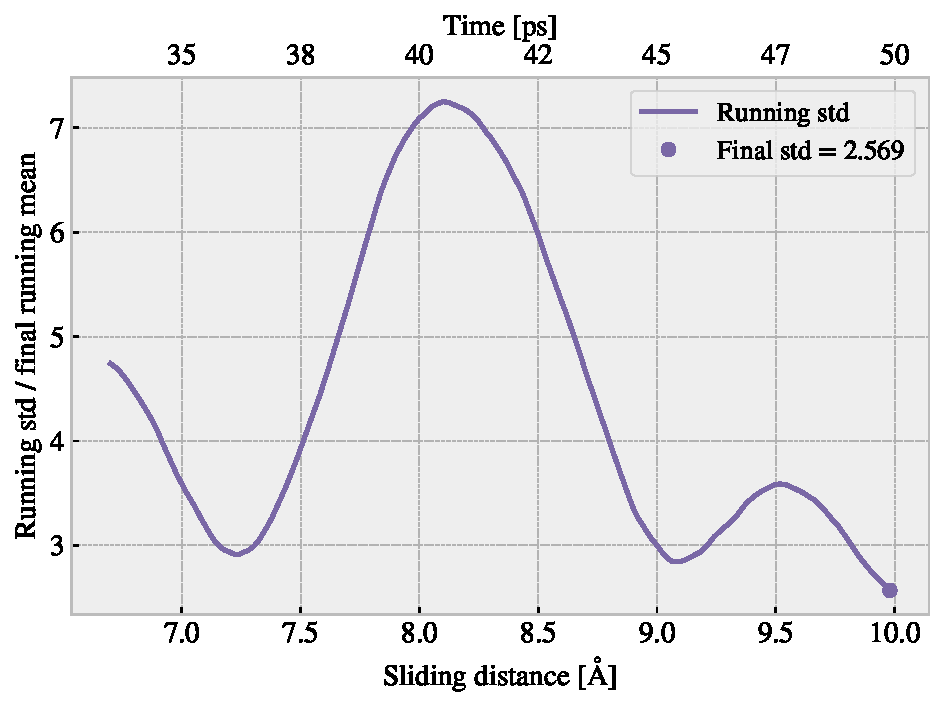
\includegraphics[width=\textwidth]{figures/baseline/Ff_runstd.pdf}
      \caption{Running std with window length $\SI{1.75}{\text{Å}}$ (35\% the mean window length.)}
      \label{fig:runstd}
  \end{subfigure}
  \caption{Running mean (a) and running relative error (std) (b) on the friction force data from a reduced sliding distance of \SI{10}{{\text{Å}}}. The running mean window is 50\% the data length while the running std window is 35\% the running mean window length. The values are plotted at the end of their respective windows such that windoe precredes the actual point on the graph.}
  \label{fig:running}
\end{figure}

When including the full dataset of 400 Å of sliding, such that the \acrshort{std} window actually matches with the longest period of oscillations expected, we get a final relative error of $\sim 12 \%$ as shown in fig \cref{fig:runstd_long}. This is arguable just at the limit of an acceptable error, but as we shall see later on in \cref{sec:load_and_stretch} this high relative error is mainly associated with the cases of low friction. When investigating different configurations under variation of load and stretch we see a considerable lower relative error as the mean friction evaluates to higher values. One interpration of this finding is simply that the oscillations in the running mean are to some degree independent of the magnitude of the friction. In that case, the relative error will spike for the low friction cases, and the absolute error might be there more reliable measure, i.e.\ taken simple the \acrshort{std} without dividing by the final mean value.


\begin{figure}[H]
  \centering
  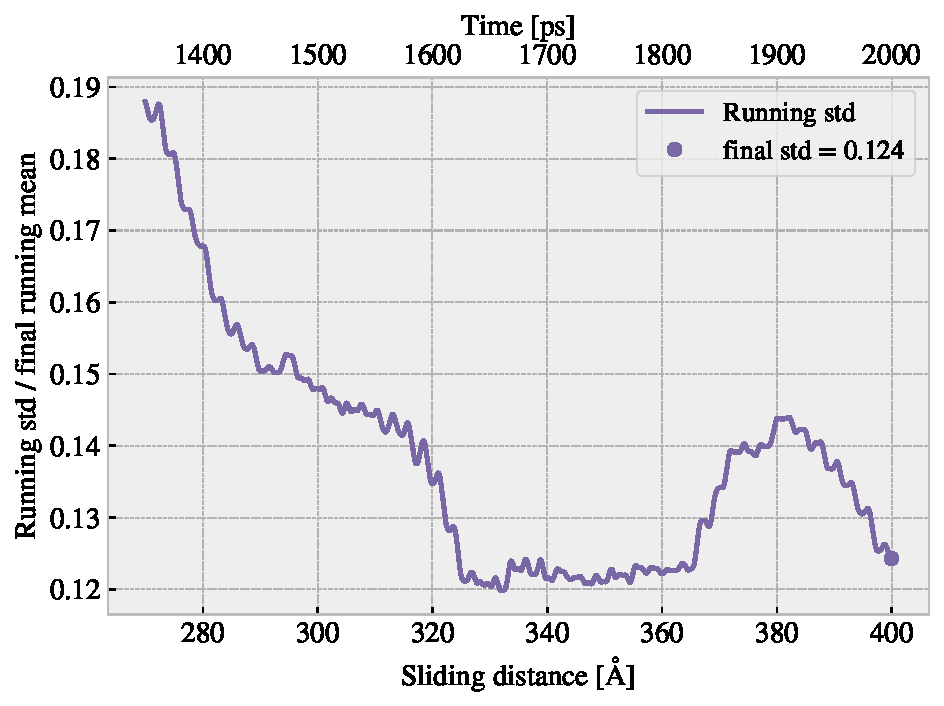
\includegraphics[width=0.6\linewidth]{figures/baseline/Ff_runstd_long.pdf}
  \caption{Running standard deviation (std) for a full \SI{400}{{\text{Å}}} sliding simulation. The running std window is 70 Å (35\% the running mean window of 50\% the data length).}
  \label{fig:runstd_long}
\end{figure}


\subsection{Static friction} 
The maximum value is one of the common choices for addressing static friction,
even though the definition of static friction is a bit vague. When considering
the force traces in \cref{fig:drag_Ff} we observe that the force oscillations
increase in magnitude toward a global peak at $\sim \SI{20}{\text{Å}}$. Thus,
one could be inclined to identify this peak as the maximum value associated with
the static friction force. However, as we have already clarified, this steady
increase in friction is a part of a slower oscillation which repeats by a period
of $\sim 71$ Å$^{-1}$. By plotting the top three max values recorded during a
full 400 Å simulation, for 30 logaritmicly spaced load values in the range
$[0.1, 100]$ nN, we observe that the global max in fact rarely fall within this
first oscillation period as shown in \cref{fig:max_dist}. Only 2 out of 30 global
maxima and 4 out of 90 top three maxima can be associated to the start of the sliding
by this definition. Thus, this result suggest that our default system does not
yield a static friction response in the sense of an initial increase in friction
due to a depinning of the sheet from the static state \hl{Is this probably
definned in the theory section}. Some parameter changes that might increase the
likelihood of seeing a significant static friction response is either extending
the relaxation period, since static friction is theorized to increase logaritmically
with time, or to increase the sliding force more slowly and through a soft spring tethering. As an attempt to test parts of this hypothesis we run a series of simulations with varying spring constant, $K\in [5, 200]$ nN including also $K = \inf$, but keeping the relaxation time and sliding speed at the default values. The result is shown in \cref{fig:max_vs_K}. The results do not show any support of the hypothesis that a softning of the spring constant will eventually lead to the maxima occouring in the first periode of sliding. We note that this might be suppressed by having a too short relaxation period or a too high sliding speed, related to the rate of which force increased initally, but due to the ambiguousness in the assesment of the static friction we will mainly concern ourselves with the kinetic friction in the remaming of this thesis.



% In most numerical studies \cite{bonelli_atomistic_2009, zhu_study_2018} they define static friction as the max peak or top 5\% quantile throughout the simulation and do not consern themselves with a requirement for an initial increasement toward this max. Thus, we interpret this as a measure of the force oscillation magnitude which is highly related to the stick-slip behaviour. 



% that the max value cannot be used as a reliable measure for the
% static friction either due to its lack of presence or due to the simulation
% setup procedure. For a more typycal evaluation of the static friction force one
% would increase force slowly until the first slip significant slip is recorded (a
% series of precursors is expected to precede this). In our simulations we drag
% the sheet relatively fast in a rigid manner which might be the reason for the lacking the static friction. Bonelli et al.\ \cite{bonelli_atomistic_2009} reported that the stick-slip behaviour was only presented when using a relatively soft spring. Thus, by changing the spring constant we investigate possibility to observe a static friction (\hl{I kind of interchanged stick-slip and static friction int his argument, but I still think it can be used to argue for doing the test...}) response within the framework of our simulation procedure as shown in
% \cref{fig:max_vs_K}. However, the results do not indicate any implications
% that a recognizable domain exist for which the static friction response would be
% reliable. Hence, we will base the final assesment on frictional properties purely on the kinetic friction force. 


\begin{figure}[H]
  \centering
  \begin{minipage}{.47\textwidth}
    \centering
    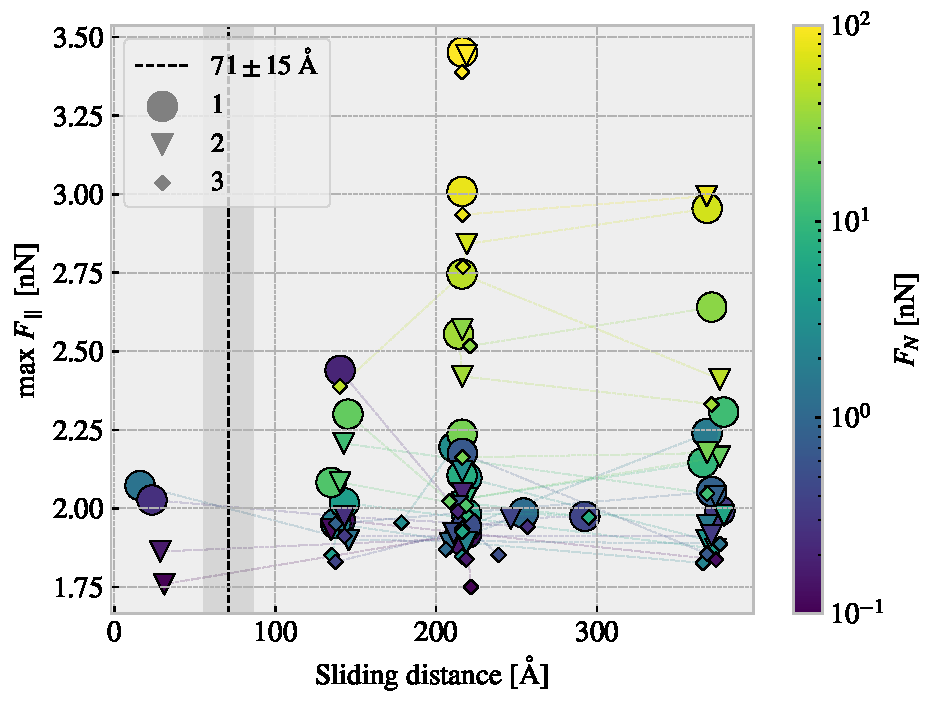
\includegraphics[width=\linewidth]{figures/baseline/max_dist.pdf}
    \captionof{figure}{Distribution of top three max friction force peaks for 30 uniformly sampled normal forces $F_N \in [0.1, 10]$ nN. The dotted line and the grey area marks the slowest significant oscialltion period found in the data and thus marking a dividing line for whether a peak falls within the ``beginning'' of the sliding simulation.}
    \label{fig:max_dist}
  \end{minipage}%
  \hspace{0.2cm}
  \begin{minipage}{.48\textwidth}
    \centering
    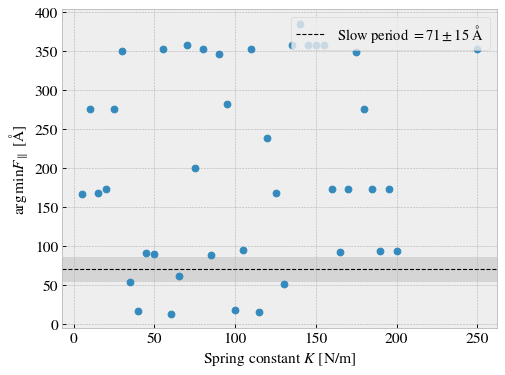
\includegraphics[width=\linewidth]{figures/baseline/max_vs_K}
    \captionof{figure}{Sliding displacement for the max friction peak to appear as a function of spring constant. \hl{Fixmove is tmp mapped to K = 200 here without any discontinuous lines.}}
    \label{fig:max_vs_K}
  \end{minipage}
  \end{figure}




% We investigate the placement of the max values, i.e. the sliding distance length for which we measure the max friction force. We show the placement of the top three max values for different simulatiosn with varying normal force in \cref{fig:max_dist}. We observe immediately that only a few top three max values is measured within a full slow period of $\sim$ 71 Å. In fact many max values is measured just before the end of the simulation. This indicates that the naive approach of using the overall max value to describe the static friction coefficient might be a to naive approach. Another approach is to use the max value within a single period, but we do not really know if this period will be similar for alle cut patterns and thus this might be limiting. 



% Look into static friction when having a spring connected to the drag force with
% rather low spring constant. Maybe compare to critical sitffness in FK model.
% Some rough calculations follow here (make a note about this being a very naive
% approach to determine a suitable stiffness for static friction scenarious. In
% reality one should increase force slowly to observe this probably). When
% dragging the sheet in the y-direction we effectively have a lattice spacing
% \begin{align*}
%   a_c = a_{2,x} + B_x = a_G\frac{\sqrt{3}}{2} + \frac{a_G}{2\sqrt{3}} = \frac{2a_G}{\sqrt{3}}
% \end{align*}
% for graphene lattice constant $a_G = 2.46$ Å. For the diamond silicon structure
% this is essentially equal to the lattice constant $a_D = 5.4210$ Å. This gives 
% \begin{align*}
%   \theta = \frac{a_c}{a_b} = \frac{2}{\sqrt{3}}\frac{a_G}{a_D} \approx 0.5230.
% \end{align*}
% Since we have the factor $2/\sqrt{3}$ it is safe to assume that this is a
% irrational number leadning to incommensurability. The worst case scnario of
% incommensurability (where $\theta$ equals the golden-mean, Can we get the exact
% number?) gives the minimal critical stiffness $K_c \sim 2U_0
% (\frac{\pi}{a_b})^2$, where $U_0$ is the substrate potentiual magnitude and
% $a_b$ the lattice spacing of the substrate. The potential barrier $U_0$ can be
% approximated by the work done when resisting the normal force as $\sim F_N
% a_D/2$ such that the critical stiffness can be approximated to 
% \begin{align*}
%   K_c \sim 2 F_N \frac{a_D}{2} \left(\frac{\pi}{a_D}\right)^2 = \frac{F_N}{a_D}\pi^2
% \end{align*}
% With a normal force of 1 nN we get $K_c \sim 18$ N/m. Hence, we should try a
% spring constant lower than that as qualified way of determining if this is the
% reason why we do not really see static friciton in the simulation. By plotting the max position (in terms of drag length) as a function of spring constant as seen in \cref{fig:max_vs_K} we can investigate if the concept of a critical spring constant is governing this simulation. However, as I'm writing this I'm realizing that the spring constant in the model applies to the interatomic forces and not the one dragging the system.....




\section{Out-of-plane buckling}\label{sec:out-of-plane_buckling}
The out-of-plane buckling is one of the original motivations for investigating
the application of Kirigami cuts in the context of friction properties. Therefore, we perform a stretch simulation, at low temperature ($T = \SI{5}{K}$) without any substrate, in order to verify that we are able to reproduce an out-of-plane buckling with the
intended patterns described in \cref{chap:system}. For this investigation we include the non-cut sheet, the Tetrahedron $(7,5,1)$ and the Honeycomb $(2,2,1,5)$ pattern. We quantify the out-of-plane buckling by assessing the distribution of atoms along the z-direction (perpendicular to the plane) during stretching. We calculate the
mininum and maximum z-value as well as the atom count quartiles 1\%, 10\%, 25\%, 50\%
(median), 75\%, 90\% and 99\% as shown in figure \cref{fig:buckling_quartiles}. The results show significant buckling for the Tetrahedron and Honeycomb patterns in comparison to the non-cut sheet which only exhibit minor
buckling of $\sim 2$ Å which is on the same order as the lattice spacing.
Moreover, we notice that the Tetrahedron pattern buckles more in consideration
to the min.\ and max.\ peaks while the remaining quantiles actually seem to be more closely spaced than for the Honeycomb. By adressing the simulation visually, using the Open Visualization Tool OVITO, we find that this can be
attributed to fringes on the edge ``flapping around'' and thus increasing the
min.\ and max.\ values.

\begin{figure}[H]
  \centering
  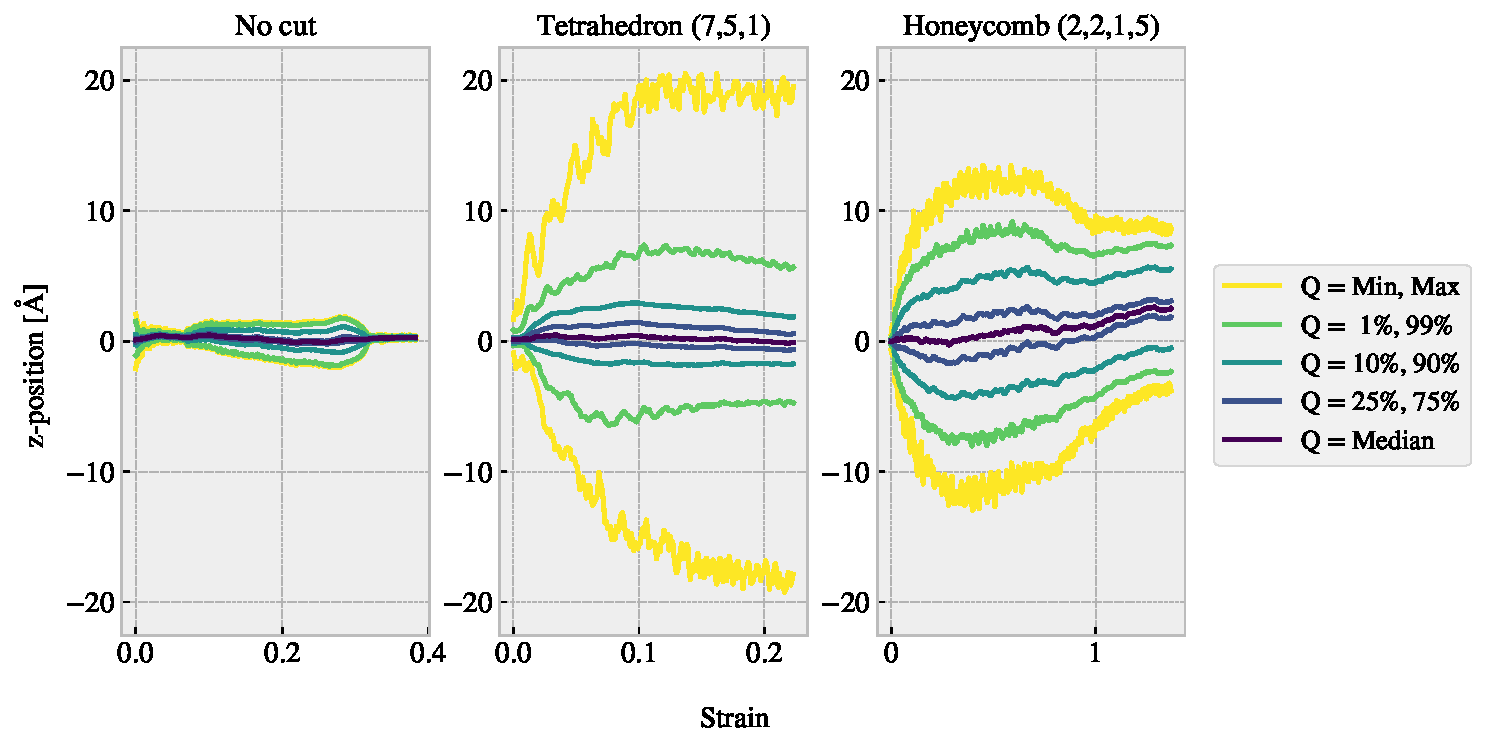
\includegraphics[width=\linewidth]{figures/baseline/vacuum_normal_buckling.pdf}
  \caption{Out-of-plane buckling during stretching of the No cut, Tetrahedron $(7,5,1)$ and Honeycomb $(2,2,1,5)$ sheet resepctively in vacuum at low temperature $T = \SI{5}{K}$. The buckling is measured by the distribution of the atom z-position (perpendicular to the sheet plane), for which the colors indicates selected quantiles. The yield strain were, reading from left to right, 0.38, 0.22 and 1.37.}
  \label{fig:buckling_quartiles}
\end{figure}

Given the confirmation of out-of-plane buckling in a vacuum, as seen in
\cref{fig:buckling_quartiles}, we reintroduce the substrate in order to
investigate whether this effect carries over to a change in contact area. We
raise the temperature to the default value of $T =\SI{300}{K}$. We keep the
normal force off and let the sheet stick purely by the adhesion forces between
the sheet and substrate. We quantify the contact area through the relative
amount of atoms in the sheet within chemical range of the substrate. The cut-off
for this interaction is set to 4 Å, inspired by \cite{li_evolving_2016},
corresponding to $\sim 120$\% the LJ equilibrium distance. Usually the contact
area is calculated as the number of contacting atoms multiplied with an
associated area for each atom. However, since we are not interested in the
absolute value of the actual area, but rather the relative change, we ommit the
multiplication factor. That is, we consider the relative number of atoms within
contact range, which is proportional to the contact area, as our metric of
choice. The relative contact for the three configurations (No cut, Tetrahedron
$(7,5,1)$ and Honeycomb $(2,2,1,5)$) during strecthing are shown in figure
\cref{fig:contact_vs_stretch}. The figure reveals a significant drop in contact
as the sheets are stretched, which agrees qualitatively with the buckling
observed without the substrate (\cref{fig:buckling_quartiles}). The Honeycomb
pattern turns out to be both the most stretchable, with a rupture strain of 1.27, and the one with the biggest decrease in relative
contact down to approximately 43\%. Notice, that the relative contact is never
actual 1.0 but instead reaches a maximum of 96\% with no stretching. This is
attributed to the temperature fluctuations and the choice of cut-off.

Selected frames from the simulation result are shown in \cref{sec:sheet_stretch}
which reveals a bit more information on how the buckling occurs. The tetrahedron pattern deforms rather quickly and smoothly into small tetrahedron
spikes, as the name suggests. In the Honeycomb pattern, on the other hand, the
deformations initiate from one side first. As the sheet stretches more rows of
the pattern are activated, producing the honeycomb-looking shape when seen from
above. Both patterns exhibit a small increase in the relative contact when they
are approaching their yield strain. This agrees with the results in
\cref{fig:buckling_quartiles} where the buckling reduces slightly towards the
end.


\begin{figure}[H]
  \centering
  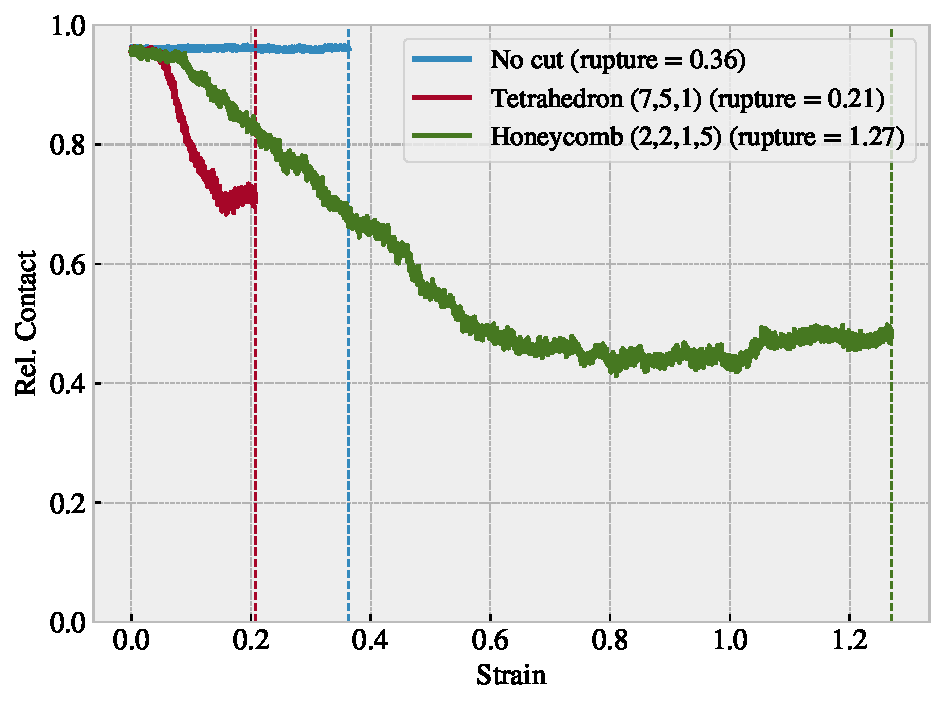
\includegraphics[width=0.6\linewidth]{figures/baseline/contact_vs_stretch.pdf}
  \caption{Relative contact, given as the relative number of atom in the sheet being within chemical interaction range, vs.\ strain of the sheet.  The cut-off for the interaction range is 4 Å corresponding to $\sim 120 \%$ the LJ equilibrium distance. No normal force is applied and temperature is kept at $T = 300$ K.}
  \label{fig:contact_vs_stretch}
\end{figure}

\hl{Compare figure} \cref{fig:contact_vs_stretch} \hl{to that of figure} \cref{fig:multi_stretch_contact} \hl{where multiple simulations constitute the stretch-contact curve.}


\section{Investigating default parameters}\label{sec:main_params}
We carry out a more extensive investigation of the dependence on friction of the temperature $T$, sliding speed $v_{\text{slide}}$ and spring
constant $K$, and timestep $dt$. This is done partly to
understand how the dependencies relate to theoretical, numerical and
experimental results, and partly to understand how these parameters affects
the stability of our system. We use the default parameters presented in
\cref{tab:final_param} and investigate the results as we change parameters, one at a time. We keep the load at \SI{1}{nN}. We consider the mean
friction force, sampled from the last half of the simulation as described in
\cref{sec:fric_metrics}, representing the kinetic friction. The results are
presented \cref{fig:main_param}. We have indicated the absolute error visually,
defined by the \acrshort{std} as described in \cref{sec:fric_metrics}, as a
shaded area that connects linearly between data points. Generally, we notice
that the parameter dependencies differ between the graphene sheet. 

\begin{figure}[H]
  \centering
  \begin{subfigure}[t]{0.49\textwidth}
      \centering
      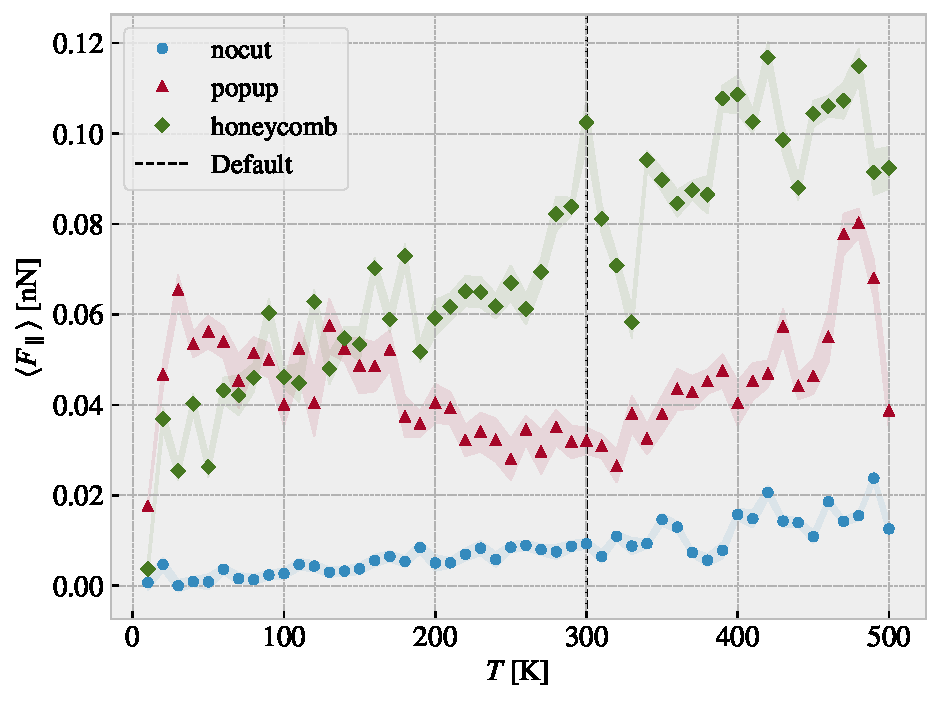
\includegraphics[width=\textwidth]{figures/baseline/variables_temp_mean_fixmove_v20.pdf}
      \caption{}
      \label{fig:var_temp}
    \end{subfigure}
    \hfill
    \begin{subfigure}[t]{0.49\textwidth}
      \centering
      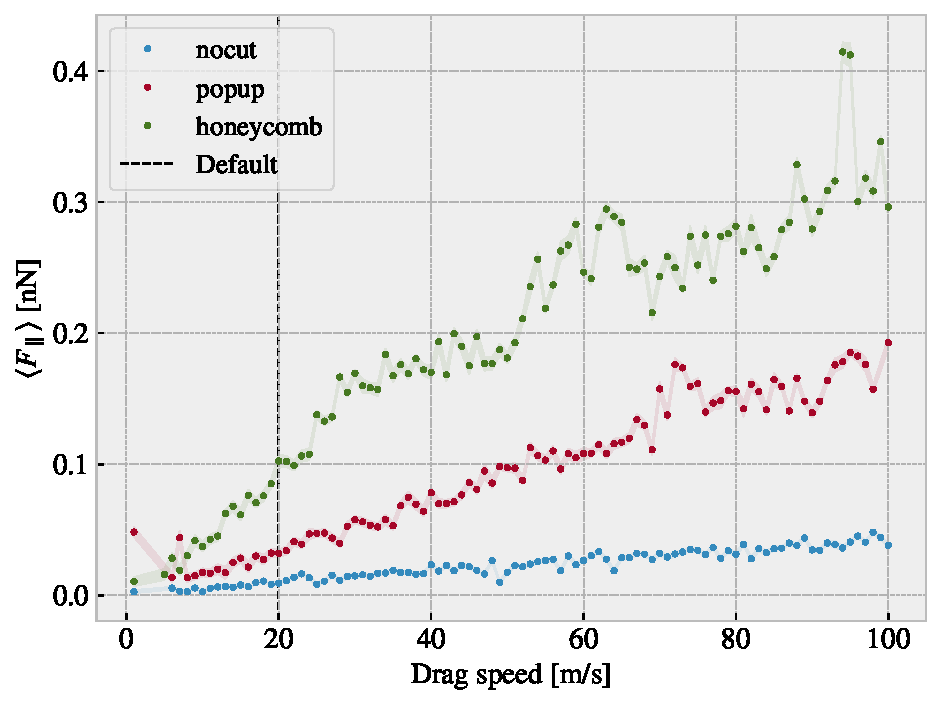
\includegraphics[width=\textwidth]{figures/baseline/variables_vel_mean_fixmove.pdf}
      \caption{}
      \label{fig:var_vel}
    \end{subfigure}
    \hfill
    \begin{subfigure}[t]{0.49\textwidth}
      \centering
      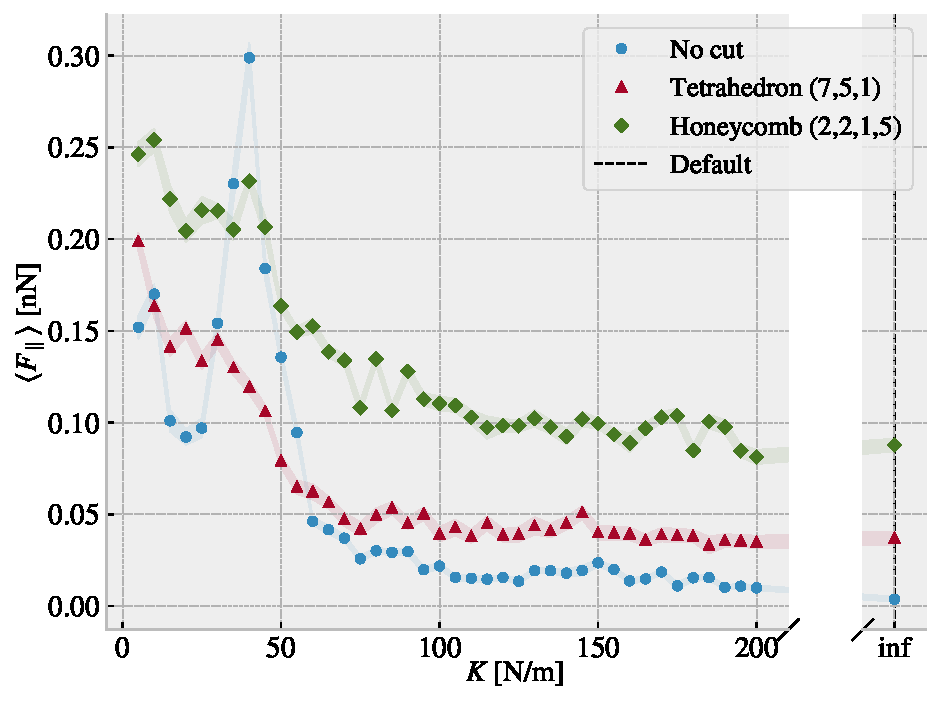
\includegraphics[width=\textwidth]{figures/baseline/variables_spring_mean_fixmove.pdf}
      \caption{}
      \label{fig:var_K}
    \end{subfigure}
    \hfill
    \begin{subfigure}[t]{0.49\textwidth}
        \centering
        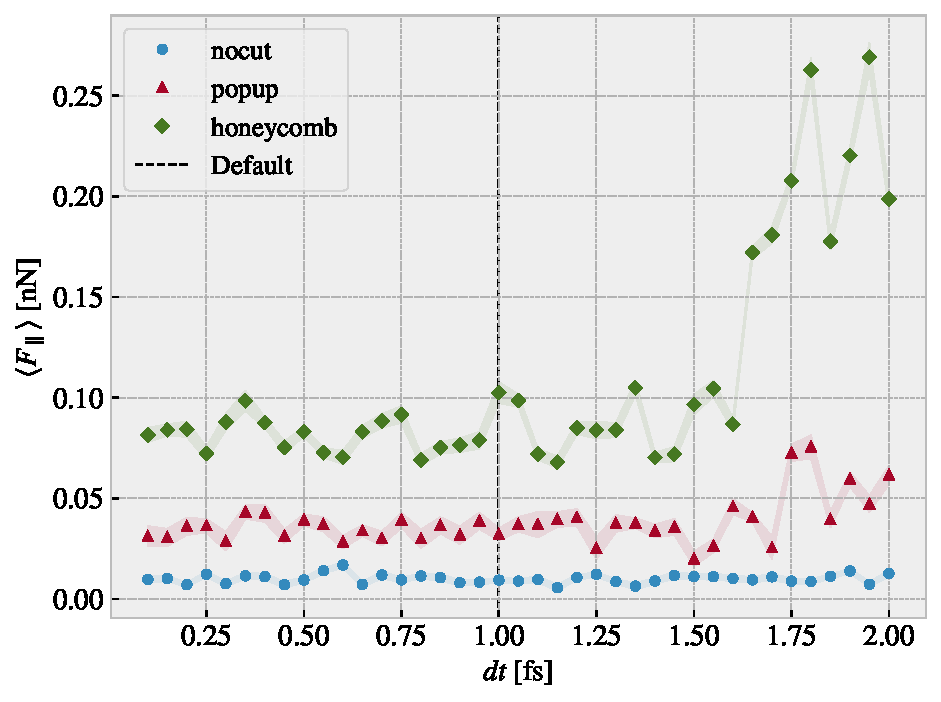
\includegraphics[width=\textwidth]{figures/baseline/variables_dt_mean_fixmove.pdf}
        \caption{}
        \label{fig:var_dt}
    \end{subfigure}
    \hfill
    \caption{Main parameters investigation. Kinetic friction force}
    \label{fig:main_param}
\end{figure}

From the temperature investigation in \cref{fig:var_temp} we find an increasing
kinetic friction with temperature for both the non-cut sheet and the Honeycomb
pattern. The Tetrahedron pattern shows both decreasing and increasing trends as
it yields an initial rapid (10--30 K), followed by a more slowly decrease
(30--320 K), which turns around and increases (320--480 K), and finally a rapid
drop decrease again (480--500 K). Similar rapid changes are also seen from the
Honeycomb pattern, although the underlying trend is seemingly increasing
throughout. We notice that for the non-cut and Honeycomb sheet, which can be
attributed to some sort of underlying linear increase, the rate of increase is
higher for the Honeycomb than the non-cut sheet. From a theoretical and
experimental point of view, we would expect a decrease in friction with
temperature. \hl{Explain why}. However, an increasing trend is also observed by Zhang et al.
\cite{ma12091425} (sliding at \SI{10}{m/s}) which we associates with a high
sliding speed causing ballistic motion \hl{Revisit theory on this one}. Since
the results does not indicate any plateau for which the temperature choice is
more or less stable with respect to changes, we have choosen the room
temperautre $T = \SI{300}{K}$ 

% For the max friction dependencies we generally also see an increasing trend with increasing temperature. This however, can be attributed to the fact that the possibilities of exiting the sheet to produce a peak force increases with temperature. 

From the sliding speed investigation in \cref{fig:var_vel} we generally find an increasing friction with velocity. Due to the relatively high velocities availble and the effects from the thermostat, we expect a viscous friction $F_k \propto v_{\text{sliding}}$ which matches rather well with these results. However, the Tetrahedron and Honeycomb sheets seem to fall slightly into a sublinear relationship as it approaches higher velocities. Moreover, the cut sheets exhibit some local fluctuations which might be attributed to resosnance effects as discussed with respect to the phonon dynamics. Our choice of sliding speed at \SI{20}{m/s} mainly reflects a consideration of computational cost, but the fact that no immediate resonance fluctuations appears around this values supports the choice.  

From the investigation of the spring constant parameter in \cref{fig:var_K} we observe a significant decrease in friction as the springs stiffens. This can be attributed to the transistion from a stick-slip influenced regieme to a smooth sliding regime as we saw for the force traces in \cref{fig:drag_Ff}. For soft springs the result is quite sensitive to the specific choice of spring constant which is especially seen for the non-cut sheet as is peaks at $K = \SI{40}{N/m}$. Thus, in order to avoid such a sensitivity we settled for the infinitely stiff spring with the intention of getting more stable results in our configuration investigation.


Finally, we consider the stability of the result as we vary the simulation timestep in \cref{fig:var_dt}. The general trend shows a stable plateau below $\sim \SI{1.5}{fs}$ for which higher values reveals arrising unstabilities for the cut sheets. This mainly confirms that our choice of timestep is within a reasonable range. However, we do see some fluctuations which are more
significant for the cut patterns. These fluctuations can be taken as a sign of the role of randomness in our simulation. An extended study of the effect of changing the random seed for the initial velcoity and thermostat could bring more insight into this matter. However, we might interpret this as an indication that the uncertainity is higher than otherwise estimated by the running mean and running \acrshort{std} evalulation. For the Honeycomb sheet the fluctuations are on the order $\pm 0.017$ which corresponds to a relative error of $\sim 20\%$. This number is a bit unsettling, but we take note of this as an upper limit for the error at an unstretched stage. 








% Quick thoughts:
% \begin{itemize}
%   \item Temperature: We do clearly not see the $1/T$ temperature decrease. The non-cut sheet seems to showcase a lienar relationship which is also somewaht present for the honeycomb which matches some of the findings in other MD simulations. For the popup we do see a local decrease at low temperatures which flip at around the default $T = \SI{300}{K}$ temperature. The max friction peaks seem to increase with temperatur as well indicating that the peaks might be associated with thermal fluctuations rather than actual stick-slip behaviour. This supports the finding that the static friction response is not significantly present in these simulations. 
%   \item Velcotiy: Considering the non-cut sheet first the velocity dependency is seemingly linear which deviates from the expected logaritmic trend. For the cutted configurations we find some peaks which might indicate the presence of resonance frequencies. The cutted sheet might be closer to a logaritmic trend, but this is not spot on either. The max friction seems to decrease slightly with small velcoties and then stay rather constant. This can probably be explained by the reduced time to stick between stick slip. 
%   \item Spring constant: On all three configurations the kinetic friction decreases with an increasing spring constant. The best explanations might be due to the lack of freedom to ``get stuck'' in incommensurable configurations. We also notice that the friction varies a lot at lower spring constants supporting the choice of having a stiff spring for stability reasons. Especially the non-cut sheet peaks at $K = \SI{40}{N/m}$. The max friction seem to be constant with $K$.
%   \item $dt$: The kinetic friction is relatively stable around the default choice of $dt = \SI{1}{fs}$. However, the fluctuations with respect to $dt$ is more significant for popup pattern and even more for the honeycomb pattern. This indicates that the more complex kinetics of the simulation is more sensitive to the timestep. We might interpret this information as an additional measure of uncertainty. The maximum friction decreases with increasing timestep which can be asserted a statistical interpretation: Higher peaks will be captured by the high resolution of a low $dt$ and vice versa. The high max values towards the point of $dt = \SI{2}{fs}$ is most likely due to the approach of unstability in the simulation as seen more clearly for the kinetic friction evaluation. 
% \end{itemize}



\subsection{Computational cost}
\hl{Say something about how we run the simulations?}

As we analyse the numerical and physical dependencies in the system we also
consider the computational cost. This especially relates to the parameters
defining the total number of computations such as timestep, sliding speed and
sliding distance. As an extension of the analysis in \cref{sec:main_params} we
report on the computational times associated with temperature, sliding speed,
spring constant and dt. By retrieving the computational time used for the
parameter investigation in \cref{fig:main_param} we get the timing as shown in
\cref{fig:comp_cost}. Note that these timings only give one time estimate for
each parameter setting as opposed to an average over multiple runs which is
nessecry for more reliable data. 


\begin{figure}[H]
  \centering
  \begin{subfigure}[t]{0.49\textwidth}
      \centering
      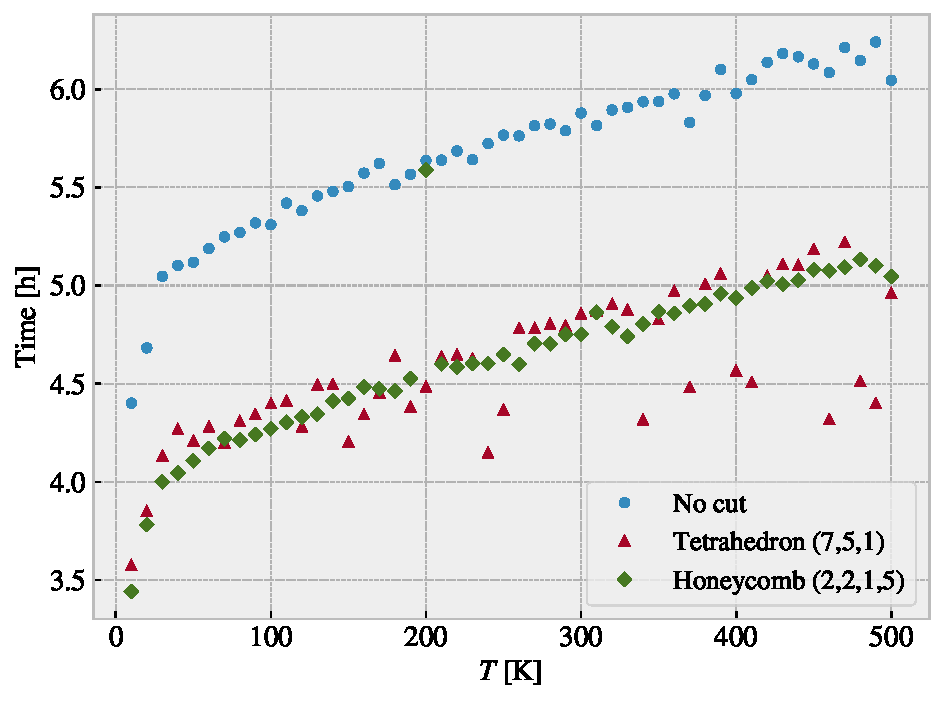
\includegraphics[width=\textwidth]{figures/baseline/comp_cost_temp.pdf}
      \caption{}
      \label{fig:comp_temp}
    \end{subfigure}
    \hfill
    \begin{subfigure}[t]{0.49\textwidth}
      \centering
      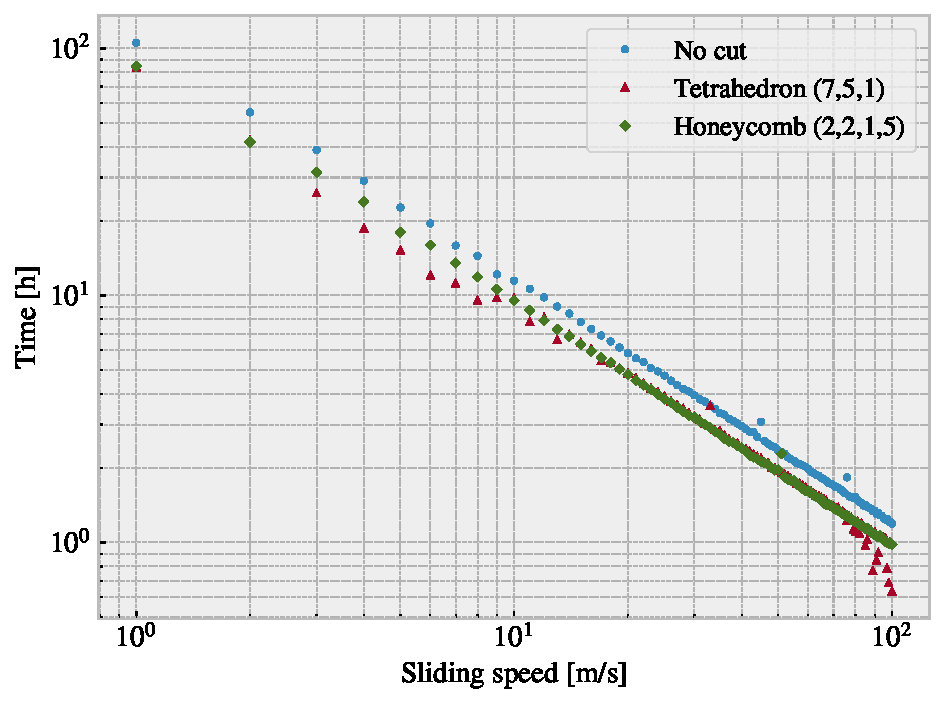
\includegraphics[width=\textwidth]{figures/baseline/comp_cost_vel.pdf}
      \caption{}
      \label{fig:comp_vel}
    \end{subfigure}
    \hfill
    \begin{subfigure}[t]{0.49\textwidth}
      \centering
      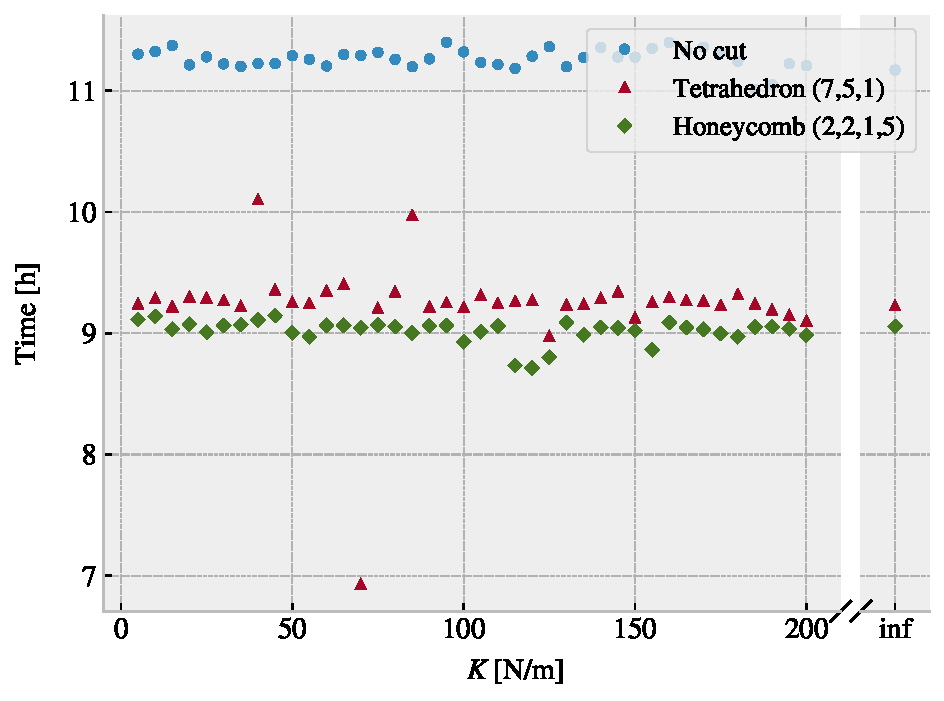
\includegraphics[width=\textwidth]{figures/baseline/comp_cost_K.pdf}
      \caption{}
      \label{fig:comp_K}
    \end{subfigure}
    \hfill
    \begin{subfigure}[t]{0.49\textwidth}
        \centering
        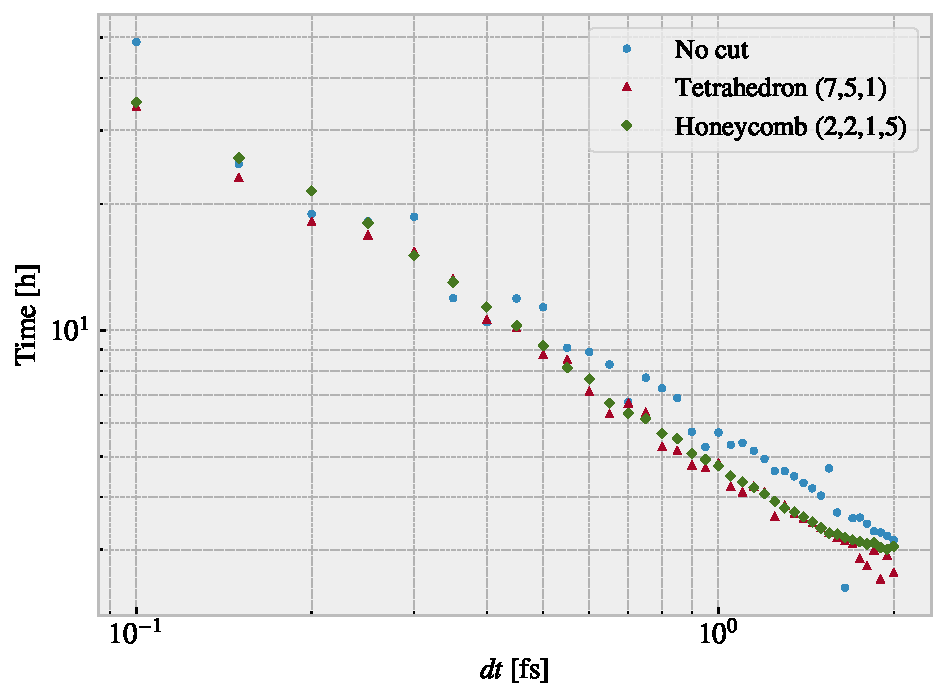
\includegraphics[width=\textwidth]{figures/baseline/comp_cost_dt.pdf}
        \caption{}
        \label{fig:comp_dt}
    \end{subfigure}
    \hfill
    \caption{Computational cost related to temperature, sliding speed, spring
    constant and dt parameter in terms of CPU hours running on 16 cores on the
    cluster \hl{double check and elaborate}. Sliding speed follows $t \propto
    v^{-0.977 \pm 0.005}$ and dt follows $t \propto \text{dt}^{-0.87\pm 0.02}$}
    \label{fig:comp_cost}
\end{figure}

The computational time is governed by the number of timesteps in the simulation
and the time used per timestep. For a fixed sliding distance, which is the case
here, the number of timesteps in the simulaiton should be inversely proportional
to sliding speed and similar inversely proportional to timestep $dt$. From the
timings in \cref{fig:comp_cost} we find the slinding speed to obey this
expectation rather well by $t \propto v^{-0.977 \pm 0.005}$ while the timing did
not increase as strongly with timestep, falling below the 1/dt relation with $t
\propto \text{dt}^{-0.87\pm 0.02}$. Moreover, we find that increasing
temperature also makes for an increased computation time. This can be attributed
to a increase in computation time associated with the force calculations. The
rising temperature give rise to more fluctuations in the system which might
yield more atoms within the force calculation cutoff's. The consideration to
cuttoff could also be part of the reason for the deviating timing relation for
$dt$. Finally, for the spring parameter, we did not see any noticable effect on
timing.



\hl{Henrik: Summarize the result of 6.5. What were the considerations, and what were the results in terms of simulation parameters?}


% Show how the number of cores per simulation scale to argue that running on just one core (maybe 4) is smart for the next step of many simulations. 

% Mention the trouble with GPU to show that this was considered, and in fact this was the reason for choosing the Tersoff potential over the AIREBO which is perhaps more common these days...



\section{Load and stretch dependencies}\label{sec:load_and_stretch}

So far, we have carried out a general analysis of the system behaviour under
different parameters which lays the foundation for the remaining study. We now
shift our intention towards the friction dependence of load and stretch.

\subsection{Pressure reference for normal load}
% source 1: stiletto heeled shoes with less than 1cm diameter:
% https://www.researchgate.net/publication/342223559_How_the_stiletto_heeled_shoes_which_are_popularly_preferred_by_many_women_affect_balance_and_functional_skills

We consider a load range of 0.1--\SI{10}{nN} which alligns with the general choice in other \acrshort{MD} studies \hl{SOURCE}. In order to relate to the magnitude of this load we provide a short calculation of the corresponding pressure. We will use the pressure underneath a stiletto heeled shoe as a high pressure reference from our macroscale world. The diameter of a stiletto heeled
shoe can be less than 1 cm \cite{stiletto_1}, and hence an \SI{80}{kg} man\footnote{Yes, a man can certainly
wear stilleto heels.} standing on one stiletto heel, with all the weight on the heel, will correspond to a pressure
\begin{align*}
  P = \frac{F}{A} = \frac{mg}{r^2\pi} = \frac{\SI{80}{kg} \cdot \SI{9.8}{\frac{m}{s^2}}}{(\frac{\SI{e-2}{m}}{2})^2 \pi} = \SI{9.98}{MPa}.
\end{align*} 
The fact that the pressure under a stiletto heel can get this high, actually greater than the pressure under an elephant food, is in an interesting realization in itself that is often used in
introductory physics courses \cite{stiletto_2}, but this also serves as a reasonible upperbound for human executed pressure. With
a full sheet area of $\sim\SI{21e3}{{\text{Å}}^2}$ our load range of 0.1--\SI{10}{nN} corresponds to a pressure of 0.47--\SI{47}{MPa} which relates nicely with our macroscale reference. This pressure might be incompatible with various industrial purposes, but with no specific application in mind this serves as a decent reference point. Notice that if we consider a human foot with area $\SI{113}{cm^2}$ \cite{stiletto_3} the pressure
drops to a mere $\SI{70}{kPa}$ corresponding to only $\sim \SI{0.01}{nN}$.

% source 3: foot area ≈ 113 cm^2:
% https://www.footbionics.com/Patients/Foot+Facts.html source 4:
% https://hypertextbook.com/facts/2003/JackGreen.shtml




\subsection{Stretch dependencies}\label{sec:stretch_dependency}
We consider the effects of stretching the sheet using the non-cut, Tetrahedron $(7,5,1)$ and Honeycomb $(2,2,1,5)$ sheet as used so far. For each configuration, we run a rupture test where the given sheet is stretched under zero load, but still under the influence of adhesion from the substrate. The rupture strain is then recorded, and multiple new simulations are initiated with strain values between zero and the rupture strain. For the sampling of the stretch values in the available range, we use a pseudo-uniform distribution, meaning that we divide the given interval into equal segments and pick a value from each segment by a uniform
distribution. This is due to numerical limitations in LAMMPS\footnote{In LAMMPS, we sample the various strain values by storing restart files during the straining of the sheet. The restart values are stored at specific timesteps governed by a LAMMPS variable. Such variables allow for a vector of uniform randomly chosen values, but unfortunately, we are not able to sort the vector for ascending values. This will lead to the script waiting to store each restart file according to the timesteps in the unsorted vector. As soon as the next timestep value is less than the current timestep the program will stop producing restart files and thus skip most of them. However, by first defining a series of intervals we can draw a uniform number for each interval without getting into trouble.}, but we find that this gives evenly spaced values which also carry some randomness. For the load we use 0.1, 1 and \SI{10}{nN}.


First, we aim to reproduce the contact investigation from
\cref{fig:contact_vs_stretch}. We quanitify the relative contact as described in
\cref{sec:out-of-plane_buckling}, but converts this into a single metric for a given simulation by considering the average of the last 50\% of data points, similar
to what we have done for the mean friction, and we adopt the same
method for quantifing the error. The results are shown
in \cref{fig:contact_vs_stretch} where we observe a significant decrease in
contact for the kirigami patterns which qualitatively agrees with the non-loaded
continous stretch investigation from \cref{fig:contact_vs_stretch}. This result implies that the change in contact can not be related to a momentum effect during stretching, as each simulation now keeps the stretching constant throughout the simulation. The absolute error for the
mean rel.\ contact were generally quite low on the order of $0.01$ for all configurations. 

From an asperity theory point of view this reduction in contact is theorized to induce a similar reduction in friction, but when considering the kinetic friction shown in \cref{fig:multi_stretch_mean_fric} we find that this is definitely not the case. As the contact decreases, for the Tetrahedron and Honeycomb pattern, the friction increases. Yet, these are not simply inversely proportional. The friction force suddenly dips down and up again, around 0.08--0.11 for the Tetrahedron and 0.73--1.05 for the Honeycomb pattern. This
suggests that the contact area is not a dominating mechanism for friction in this
system. The absolute error for the mean friction measure was fairly low on the order of 0.001--\SI{0.01}{nN}.

We notice also that the two orders of magnitude increase in normal load
did not make a significant difference in the results. In a study by Zhang et al.\ \cite{zhang_tuning_2019} they found that straining the sheet lead to a reduction in friction. Despite the fact that our result suggest an increase in friction with straining we notice that the observed effect is only present for the kirigami sheets, while the friction force on the non-cut sheet shows no appreciable dependency on the stretching.


% Tension does also not seem to be the answer since the non cut sheet does not really change 






% Regarding the contact this can be attributed the fact that load is applied to the pull blocks only. Thus, an
% increased load will not contribute directly to a compression of the kirigami induced
% asperities which is why the contact remains relatively uneffected by the load.
% The fact the friction does not increase considerable with load relates to the
% discussion of the load dependence for an atomically flat sheet. This is further
% investigated in \cref{load_dependency}.

% notice that the initial non stretch values also changes. No cut gives lowest friction.










\begin{figure}[H]
  \centering
  \begin{subfigure}[t]{\textwidth}
      \centering
      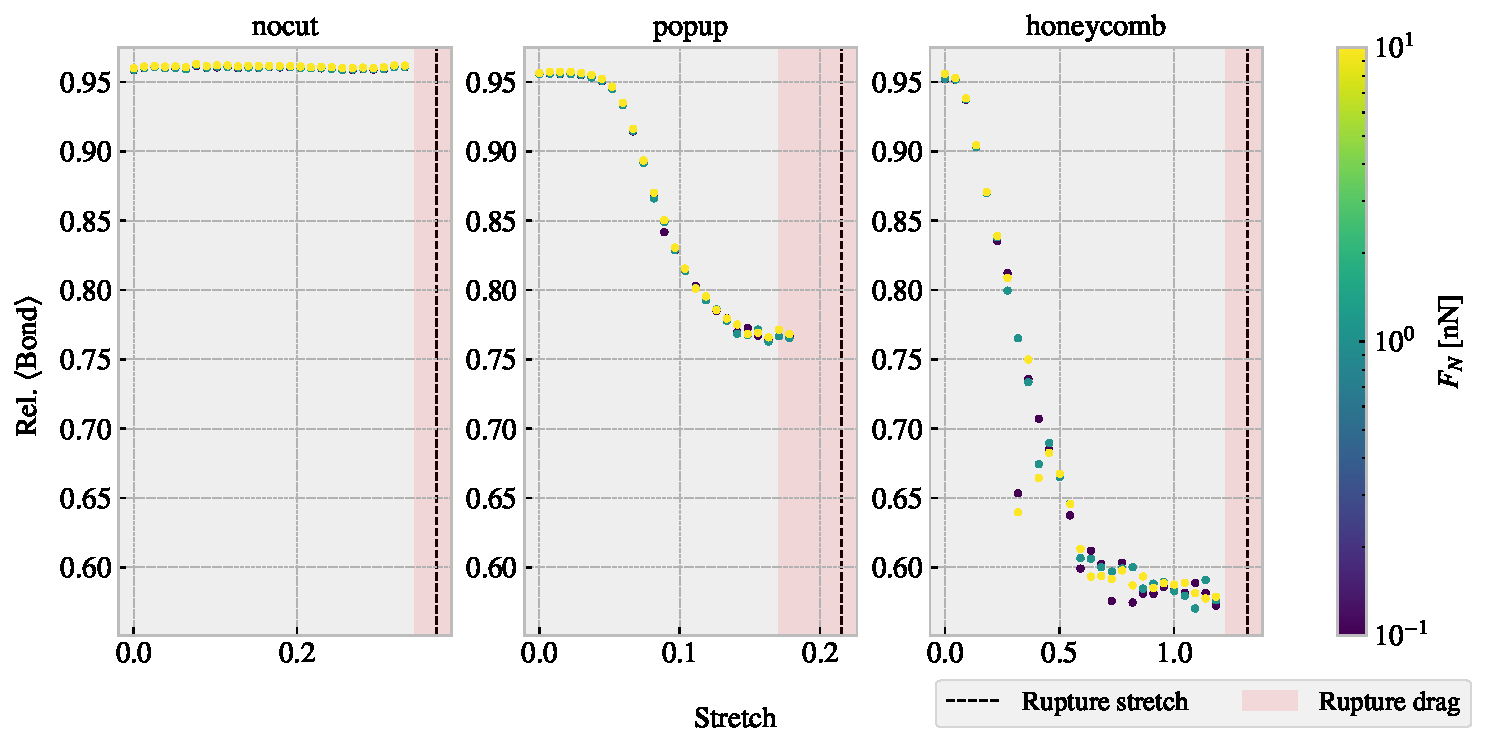
\includegraphics[width=\textwidth]{figures/baseline/multi_stretch_area_compare.pdf}
      \caption{}
      \label{fig:fig:multi_stretch_contact}
  \end{subfigure}
  \hfill
  \begin{subfigure}[t]{\textwidth}
      \centering
      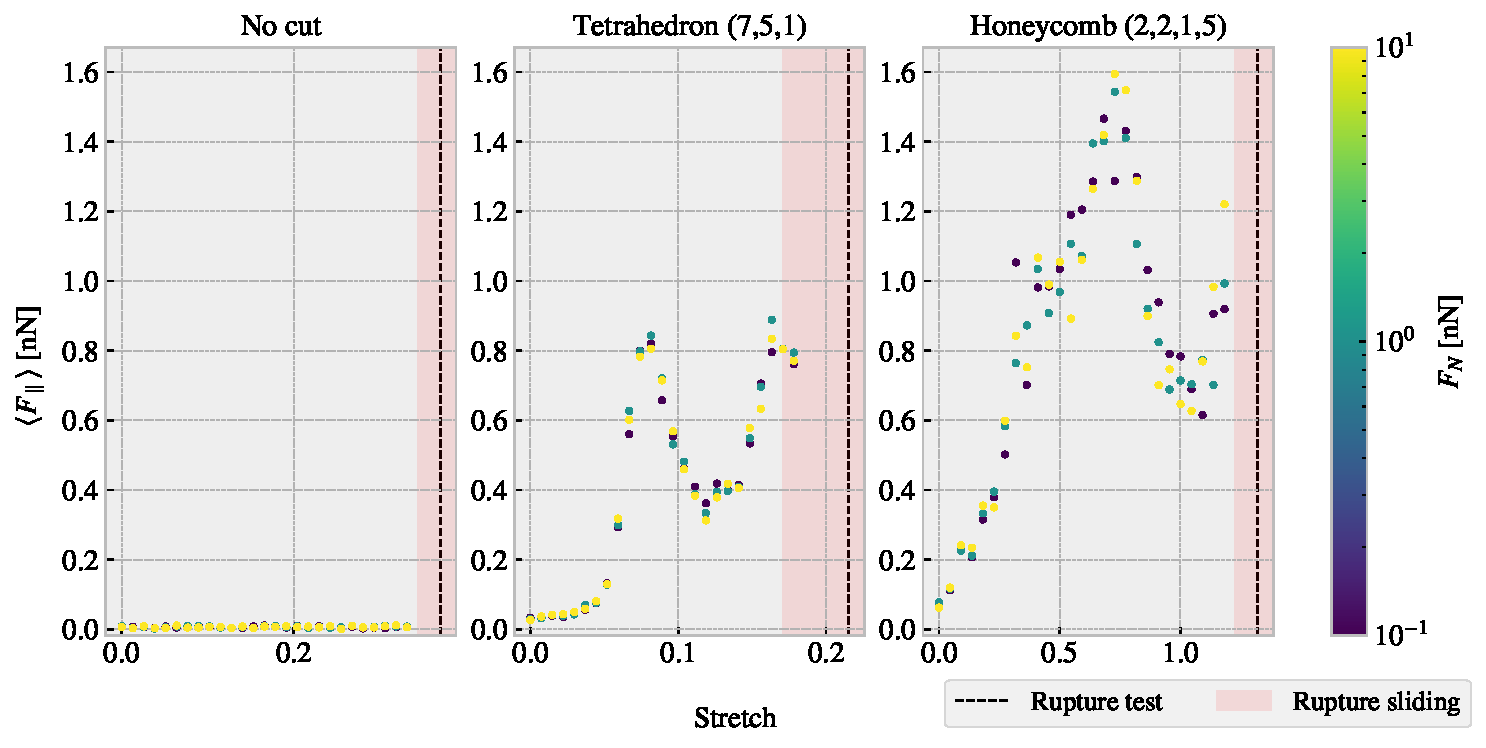
\includegraphics[width=\textwidth]{figures/baseline/multi_stretch_mean_compare.pdf}
      \caption{}
      \label{fig:multi_stretch_mean_fric}
  \end{subfigure}
  \hfill
     \caption{Average relative contact and average friction for multiple simulations, consisting of 30 stretch values sampled from a pseudo uniform distribution between 0 and the rupture point in combination with loads 0.1, 1 and \SI{10}{nN}, for each of the configurations: non-cut, Tetrahedron $(7,5,1)$ and Honeycomb $(2,2,1,5)$. The average is taken over the last half of the sliding phase. The red shade denotes the stretch range where ruptures accoured during sliding while the black-dotted line represent the rupture point in the no load rupture test. (a) The average relative contact defined as the relative number of atoms within a contact threshold of 4 Å to the substarte. The absolute error is on the order 0.01 (b) The average mean friction force parallel to the sliding direction. The absolute error is on the order 0.001--\SI{0.01}{nN}}
     \label{fig:multi_stretch}
\end{figure}

By considering the increase in friction from no stretch towards the first peak we find that the Tetrahedron pattern exhibit a relative increase of $\sim 27.7$ while the Honeycomb pattern exhibit a relative increase of $\sim 22.4$. This is in itself a remarkable result, but considering that the friction drops almost as dramatically down again is even more unexpected. These results are thus promising for the prospect of demonstrating a negaive friction coefficients by altering the stretch through a coupling to the load.


\hl{Henrik: Her kan du godt skrive litt mer. Poengtere akkurat hvor mye friksjonen faller. Og spekulere litt i hvordan man kan bruke dette til ae designe noe med negativ friksjonskoeffisient.}


% get a relative friction increase and increase vs. stretch ratios as described in \cref{tab:first_peak_stretch}. While the honeycomb force increase towards the first peak is approximately linear the popup exhibits seemingly exponential growth which yield a slope on the order $\sim \SI{30}{nN}$. 

% \begin{table}[H]
%   \begin{center}
%   \caption{(stretch, kinetic friction) coordinates from \cref{fig:multi_stretch_mean_fric} at start and the first peak respectively used to approximate the relative increase in friction force and the ratio for friction increaese vs. stretch for sait range. In practice  the latter ratio denotes the slope of a forced linear trend. }
%   \label{tab:first_peak_stretch}
%   \begin{tabular}{ | c | c | c | c | c |} \hline
%   Configuration & Start & First peak & Relative increase & Friction force vs. stretch ratio [nN]  \\ \hline
%   Popup & $\sim (0, 0.03)$ & $\sim(0.082, 0.83)$ & 27.7 & 9.76  \\ \hline
%   Honeycomb & $\sim (0, 0.07)$ &  $\sim (0.728, 1.57)$ & 22.4 & 2.06 \\ \hline
%   \end{tabular}
%   \end{center}
% \end{table}

% Additionally, we notice that booth the popup and honeycomb also exhibits stretch ranges where the kinetic friction force decrease with increasing stretch. Qualitatively we assign the slope to be on the same order of magnitude as those towrds the first peak. This is useful for the prospect of taking advantage of this phenonama as we can essentially achieve booth higher and lower friction for increasing stretch for different starting points. 


\subsection{Load dependency}\label{sec:load_dependency}
From the investigation of the stretch dependency we saw that increasing the normal load from 0.1 to \SI{10}{nN} did not make a considerable impact on the friction in comparison to the effect associated with stretch. One special feature of our system is that we only apply load to the pull blocks, and thus one might suspect this to be of importance. Therefore, we investigate the friction under varying load for a non-cut sheet comparing the case of loading the pull block against a more traditional uniform loading of the sheet as shown in \cref{fig:load_dist}. Both load distribution shows a seemingly non-dependent relationship considering the size of our estimated error. Nevertheless, we do not see any indications that the uniform loading changes the qualitative behaviour.

\begin{figure}[H]
  \centering
  \begin{subfigure}[t]{0.49\textwidth}
      \centering
      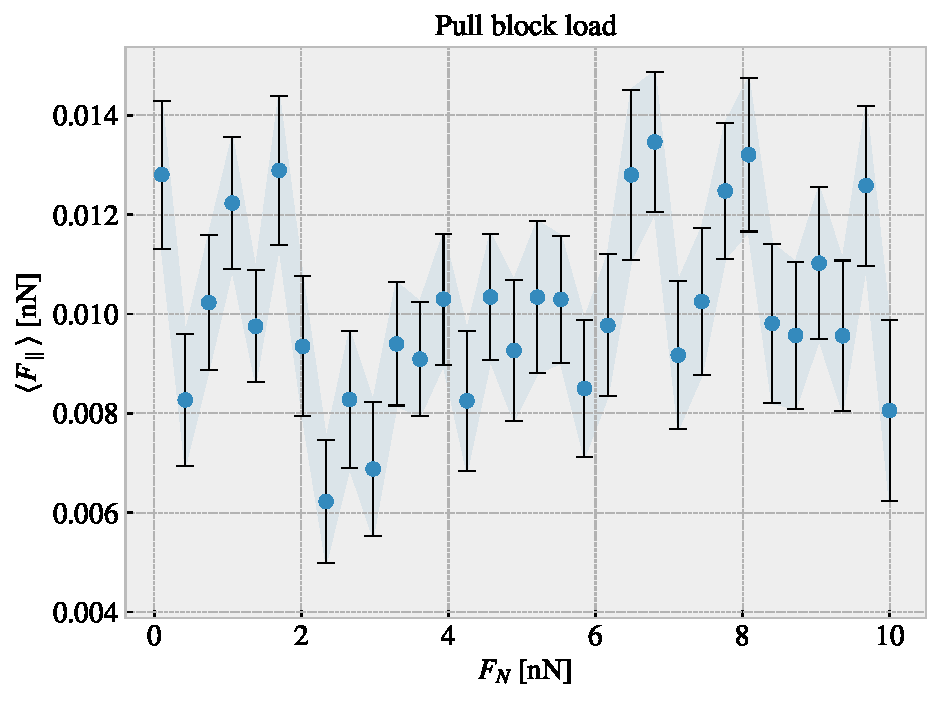
\includegraphics[width=\textwidth]{figures/baseline/load_dist_a.pdf}
      \caption{}
      \label{fig:load_dist_a}
  \end{subfigure}
  \hfill
  \begin{subfigure}[t]{0.49\textwidth}
      \centering
      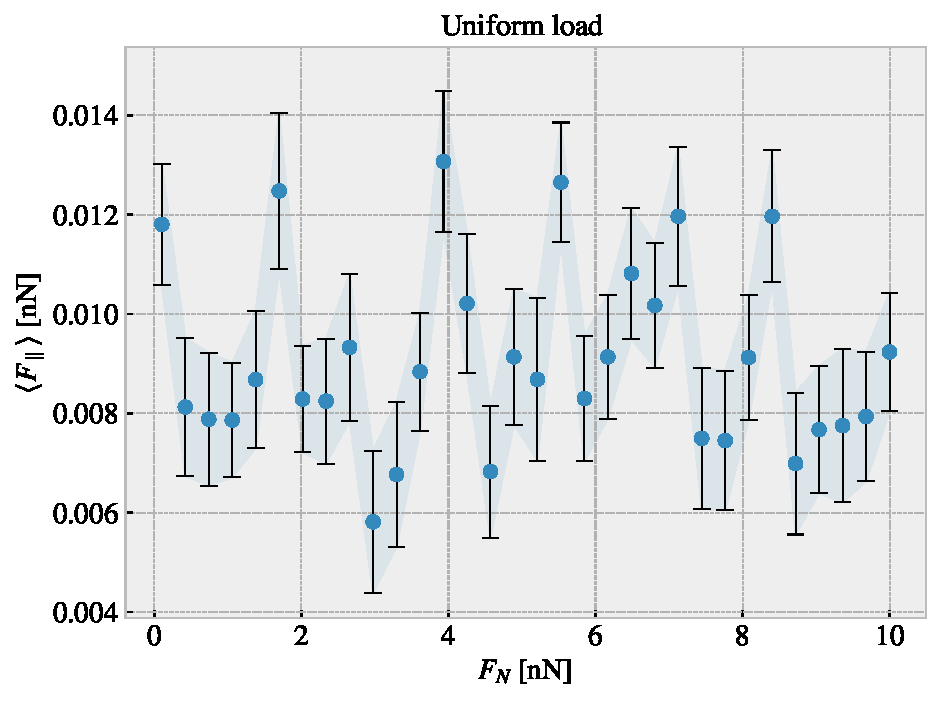
\includegraphics[width=\textwidth]{figures/baseline/load_dist_b.pdf}
      \caption{}
      \label{fig:load_dist_b}
  \end{subfigure}
  \hfill
     \caption{Multiple simulations of non-cut sheet under different load. Mean friction is plotted against load for two different variations of loading distribution. (a) Normal loading is applied to the pull blocks. (b) Normal loading is applied uniformly to the sheet. }
     \label{fig:load_dist}
\end{figure}

In order to investigate the friction dependency of normal load for the kirigami
patterns as they are stretched, we select a subset of stretch stages from
\cref{fig:multi_stretch_mean_fric} and perform additionally simulations with a
logarithmically increasing normal load in the extended range 0.1--100 nN, using
30 load points for each stretch. The results are shown in
\cref{fig:load_dependency}. Now, when spanning three orders of magnitude for
load, we start to see a noticable increase in friction. This goes for all
patterns, but it is only really visible for the non-cut sheet as the friction
axis is a lot more zoomed in. Due to the fact that we have plotted the normal
load on an logarithmic axis any seemingly linear trends on the figure is in fact
sublinear. However, as the normal load approaches 100 nN we do start to se an
increase that is more remniscent of a linear relationship, but this is difficult
to judge given that the change in friction is small in comparison to the noise
in the data. Note that we omitted the error bars for visual purposes but they
are one the same order of magnitude as shown in \cref{fig:load_dist}.


\begin{figure}[H]
  \centering
  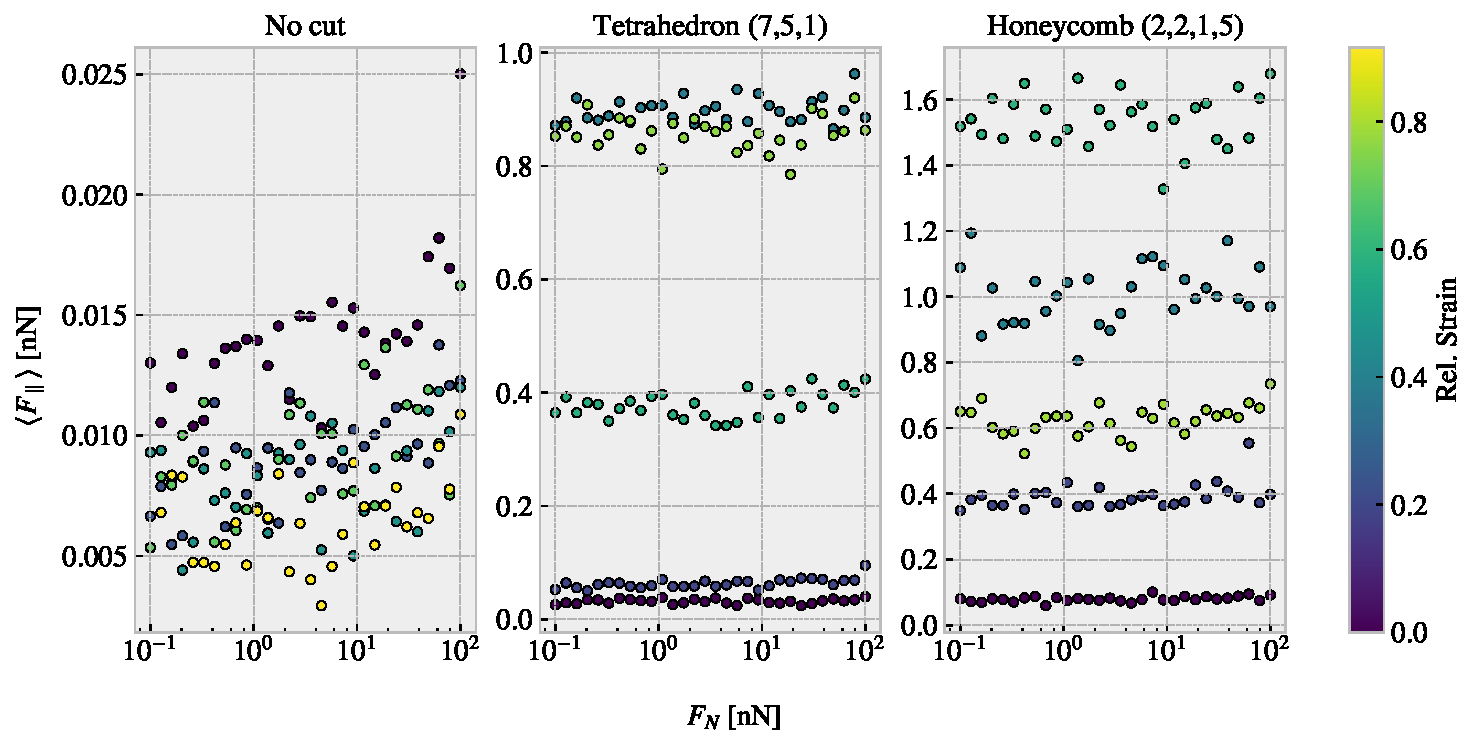
\includegraphics[width=\linewidth]{figures/baseline/multi_FN_mean_compare.pdf}
  \caption{Mean friction force vs.\ load in the range 0.1--100 nN, for the non-cut, Tetrahedron $(7,5,1)$ and Honeycomb $(2,2,1,5)$ sheet resepctively, at different stretch stages relative to their rupture point. }
  \label{fig:load_dependency}
\end{figure}

From the friction measurements in \cref{fig:load_dependency} we see that the
non-cut sheet generally produce a friction force in the order of 0.005--0.0025
nN throughout the 0.1--100 nN load range. Using a ratio based friction coeffcient definition
\cref{eq:mu_def1}, $\mu_1 = F_{\text{fric}}/{F_N}$, this would lead to a coefficient roughly in the range
\begin{align*}
  &\mu_1,  \ \text{\cref{eq:mu_def1}:}& &\text{No cut}\sim [\num{e-4}, 0.13],&  &\text{Tetrahedron}\sim [\num{4e-4},8.7],& &\text{Honeycomb}\sim [\num{9e-4}, 15.2].&
\end{align*}
However, these values mainly reflect the
poornes of this definition, as we find the values to diverge at low load and decrease towards high load due to the lacking linear relationship and an offset in the load curve corresponding to a finite friction at zero load. This offset is drastically enhanced for the kirigami patterns under applied stretch. Due to the small changes in friction compared to the noise in the data, it is not sensible to calculate the slope $dF_{\text{fric}}/dF_N$ as a function of load. Nonetheless, if we force a linear fit for the whole range and use the second definition \cref{eq:mu_def2} as $\langle \mu_2 \rangle = \Delta F_{\text{fric}}/\Delta F_N$, we get average coefficients in the range
\begin{align*}
  &\mu_2,  \ \text{\cref{eq:mu_def2}:}& &\text{No cut} \sim [4, 9]\times \num{e-5},&  &\text{Tetrahedron} \sim 5\times[\num{e-5}, \num{e-4}],& &\text{Honeycomb} \sim [1,9]\times \num{e-4},&
\end{align*}
depending on the stretch values. These numbers should be interpreted cautiously,
but we can interpret it as a rough estimate of the friction coefficient being on
the order \num{e-4}--\num{e-5}. This relates to the finding by
\cite{DIENWIEBEL2005197} who reported a seemingly non-existing relationship
between friction and normal load with change in friction that corresponds to a friction coefficients in the range \num{e-3}--\num{e-4} when using the slope definition \cref{eq:mu_def2}. This supports the idea that the graphene sheet does in fact exhibit superlubric behavior in these conditions. Moreover, the fact that the increase with load is relatively unaffected by the stretching points to the fact that the stretch-induced effect mainly shifts the load curve towards higher friction but does not significantly alter its slope. Considering the big difference
in the ratio for the demonstrated friction changes with stretch (for the
kirigami patterns) and the friction coefficients, we can conclude that the stretch-induced mechanism is dominating the friction response. This works well with the idea of creating a nanomachine that couples load and stretch. By applying load on the nanomachine we would increase both the load and the strain on the sheet simultaneously. However, since the friction dependency to strain dominates in comparison to load effects such a system can be designed entirely by considering the strain dependency.






